% Options for packages loaded elsewhere
\PassOptionsToPackage{unicode}{hyperref}
\PassOptionsToPackage{hyphens}{url}
\PassOptionsToPackage{dvipsnames,svgnames*,x11names*}{xcolor}
%
\documentclass[
  11pt,
]{article}

%Additions
\newif\iftimestamp
\timestampfalse
%

\usepackage{lmodern}
\usepackage{amssymb,amsmath}
\usepackage{ifxetex,ifluatex}
\ifnum 0\ifxetex 1\fi\ifluatex 1\fi=0 % if pdftex
  \usepackage[T1]{fontenc}
  \usepackage[utf8]{inputenc}
  \usepackage{textcomp} % provide euro and other symbols
\else % if luatex or xetex
  \usepackage{unicode-math}
  \defaultfontfeatures{Scale=MatchLowercase}
  \defaultfontfeatures[\rmfamily]{Ligatures=TeX,Scale=1}
\fi

% Use upquote if available, for straight quotes in verbatim environments
\IfFileExists{upquote.sty}{\usepackage{upquote}}{}
\IfFileExists{microtype.sty}{% use microtype if available
  \usepackage[]{microtype}
  \UseMicrotypeSet[protrusion]{basicmath} % disable protrusion for tt fonts
}{}
\makeatletter
\@ifundefined{KOMAClassName}{% if non-KOMA class
  \IfFileExists{parskip.sty}{%
    \usepackage{parskip}
  }{% else
    \setlength{\parindent}{0pt}
    \setlength{\parskip}{6pt plus 2pt minus 1pt}}
}{% if KOMA class
  \KOMAoptions{parskip=half}}
\makeatother
\usepackage{xcolor}
\IfFileExists{xurl.sty}{\usepackage{xurl}}{} % add URL line breaks if available
\IfFileExists{bookmark.sty}{\usepackage{bookmark}}{\usepackage{hyperref}}
\hypersetup{
  pdftitle={Homework 7},
  colorlinks=true,
  linkcolor=Maroon,
  filecolor=Maroon,
  citecolor=Blue,
  urlcolor=blue,
  pdfcreator={LaTeX via pandoc}}
\urlstyle{same} % disable monospaced font for URLs
\usepackage[margin=1truein]{geometry}
\usepackage{color}
\usepackage{fancyvrb}
\newcommand{\VerbBar}{|}
\newcommand{\VERB}{\Verb[commandchars=\\\{\}]}
\DefineVerbatimEnvironment{Highlighting}{Verbatim}{commandchars=\\\{\}}
% Add ',fontsize=\small' for more characters per line
\newenvironment{Shaded}{}{}
\newcommand{\AlertTok}[1]{\textcolor[rgb]{1.00,0.00,0.00}{\textbf{#1}}}
\newcommand{\AnnotationTok}[1]{\textcolor[rgb]{0.38,0.63,0.69}{\textbf{\textit{#1}}}}
\newcommand{\AttributeTok}[1]{\textcolor[rgb]{0.49,0.56,0.16}{#1}}
\newcommand{\BaseNTok}[1]{\textcolor[rgb]{0.25,0.63,0.44}{#1}}
\newcommand{\BuiltInTok}[1]{#1}
\newcommand{\CharTok}[1]{\textcolor[rgb]{0.25,0.44,0.63}{#1}}
\newcommand{\CommentTok}[1]{\textcolor[rgb]{0.38,0.63,0.69}{\textit{#1}}}
\newcommand{\CommentVarTok}[1]{\textcolor[rgb]{0.38,0.63,0.69}{\textbf{\textit{#1}}}}
\newcommand{\ConstantTok}[1]{\textcolor[rgb]{0.53,0.00,0.00}{#1}}
\newcommand{\ControlFlowTok}[1]{\textcolor[rgb]{0.00,0.44,0.13}{\textbf{#1}}}
\newcommand{\DataTypeTok}[1]{\textcolor[rgb]{0.56,0.13,0.00}{#1}}
\newcommand{\DecValTok}[1]{\textcolor[rgb]{0.25,0.63,0.44}{#1}}
\newcommand{\DocumentationTok}[1]{\textcolor[rgb]{0.73,0.13,0.13}{\textit{#1}}}
\newcommand{\ErrorTok}[1]{\textcolor[rgb]{1.00,0.00,0.00}{\textbf{#1}}}
\newcommand{\ExtensionTok}[1]{#1}
\newcommand{\FloatTok}[1]{\textcolor[rgb]{0.25,0.63,0.44}{#1}}
\newcommand{\FunctionTok}[1]{\textcolor[rgb]{0.02,0.16,0.49}{#1}}
\newcommand{\ImportTok}[1]{#1}
\newcommand{\InformationTok}[1]{\textcolor[rgb]{0.38,0.63,0.69}{\textbf{\textit{#1}}}}
\newcommand{\KeywordTok}[1]{\textcolor[rgb]{0.00,0.44,0.13}{\textbf{#1}}}
\newcommand{\NormalTok}[1]{#1}
\newcommand{\OperatorTok}[1]{\textcolor[rgb]{0.40,0.40,0.40}{#1}}
\newcommand{\OtherTok}[1]{\textcolor[rgb]{0.00,0.44,0.13}{#1}}
\newcommand{\PreprocessorTok}[1]{\textcolor[rgb]{0.74,0.48,0.00}{#1}}
\newcommand{\RegionMarkerTok}[1]{#1}
\newcommand{\SpecialCharTok}[1]{\textcolor[rgb]{0.25,0.44,0.63}{#1}}
\newcommand{\SpecialStringTok}[1]{\textcolor[rgb]{0.73,0.40,0.53}{#1}}
\newcommand{\StringTok}[1]{\textcolor[rgb]{0.25,0.44,0.63}{#1}}
\newcommand{\VariableTok}[1]{\textcolor[rgb]{0.10,0.09,0.49}{#1}}
\newcommand{\VerbatimStringTok}[1]{\textcolor[rgb]{0.25,0.44,0.63}{#1}}
\newcommand{\WarningTok}[1]{\textcolor[rgb]{0.38,0.63,0.69}{\textbf{\textit{#1}}}}
\usepackage{longtable,booktabs}
% Correct order of tables after \paragraph or \subparagraph
\usepackage{etoolbox}
\makeatletter
\patchcmd\longtable{\par}{\if@noskipsec\mbox{}\fi\par}{}{}
\makeatother
% Allow footnotes in longtable head/foot
\IfFileExists{footnotehyper.sty}{\usepackage{footnotehyper}}{\usepackage{footnote}}
\makesavenoteenv{longtable}
\usepackage{graphicx}
\makeatletter
\def\maxwidth{\ifdim\Gin@nat@width>\linewidth\linewidth\else\Gin@nat@width\fi}
\def\maxheight{\ifdim\Gin@nat@height>\textheight\textheight\else\Gin@nat@height\fi}
\makeatother
% Scale images if necessary, so that they will not overflow the page
% margins by default, and it is still possible to overwrite the defaults
% using explicit options in \includegraphics[width, height, ...]{}
\setkeys{Gin}{width=\maxwidth,height=\maxheight,keepaspectratio}
% Set default figure placement to htbp
\makeatletter
\def\fps@figure{htbp}
\makeatother
\setlength{\emergencystretch}{3em} % prevent overfull lines
\providecommand{\tightlist}{%
  \setlength{\itemsep}{0pt}\setlength{\parskip}{0pt}}
\setcounter{secnumdepth}{-\maxdimen} % remove section numbering
\ifluatex
  \usepackage{selnolig}  % disable illegal ligatures
\fi

\title{Homework 7}
\author{}
\date{May 7, 2021}

\usepackage{caption}
\usepackage{subcaption}

%-----------------------------------
\usepackage{lastpage}
\usepackage{fancyhdr}
\pagestyle{fancy}
%-----------------------------------
\makeatletter
\renewcommand{\sectionmark}[1]{%
  \markboth{%
    \ifnum\c@secnumdepth>\m@ne
      \@chapapp\ {\thesection}. \ %
    \fi
  #1%
  }{}%
}
\makeatother

%-----------------------------------
% \makeatletter
% \def\fps@figure{h}
% \makeatother

\usepackage{float}
\let\origfigure\figure
\let\endorigfigure\endfigure
\renewenvironment{figure}[1][2] {
    \expandafter\origfigure\expandafter[H]
} {
    \endorigfigure
}
%-----------------------------------

\newcommand\department{Math}
\newcommand\course{228}
%\newcommand\hwnumber{1}
\newcommand\duedate{Spring 2021}
\newcommand\NetIDa{Claudio Perez}
%-----------------------------------

\headheight 35pt
\lhead{}
%\lhead{University of California, Berkeley \\ Project \hwnumber }
%\chead{\textsc{\leftmark}}%Problem \thesection}}
\lhead{\textsc{\leftmark}}%Problem \thesection}}
\rhead{\NetIDa }
\lfoot{}
\cfoot{}
\cfoot{\small\thepage\ of \pageref{LastPage}}
\headsep 1.5em
%\title{Project \hwnumber}
%------------------------------------------------------------------
\usepackage{framed}
\usepackage{quoting}

\renewenvironment{quote}%
{%
\definecolor{shadecolor}{rgb}{0.96,0.96,0.96}%
\begin{shaded*}\quoting[leftmargin=0pt, vskip=0pt]
}%
{\endquoting\end{shaded*}}

%------------------------------------------------------------------
%------------------------------------------------------------------
\usepackage{tikz}
\input{../../style/pre}

\begin{document}
\maketitle

{
\hypersetup{linkcolor=}
\setcounter{tocdepth}{3}
\tableofcontents
}

\pagebreak

\hypertarget{problem-1.}{%
\section{Problem 1.}\label{problem-1.}}

\begin{quote}
(12 points) Solve the Dirichlet problem

\[
 \begin{aligned}
   -\Delta u &= 4, & \quad &\text{in $\Omega$} \\
           u &= 0, & &\text{on $\partial\Omega$}
 \end{aligned}
\]

on the unit disk \(\Omega=\{(x,y)\;:\; x^2+y^2\le 1\}\) using quadratic
isoparametric elements.
\end{quote}

A function implementing quadratic Lagrange interpolation over a
reference triangle is implemented in the file \texttt{interpolate.py}
which is used by the function \texttt{poisson2} from \texttt{poisson.py}
to create a finite element that locally evaluates the following
variational Poisson problem

\[
\sum_{j=1}^{n} \mathbf{u}_{j} \int_{\Omega} \nabla \phi_{j} \cdot \nabla \phi_{i}=\int_{\Omega} \phi_{i} f+\int_{\partial \Omega_{N}} \phi_{i} g_{N}-\sum_{j=n+1}^{n+n_{\partial}} \mathbf{u}_{j} \int_{\Omega} \nabla \phi_{j} \cdot \nabla \phi_{i}
\]

This is then integrated over the domain using a self-implemented system
optimization package called \texttt{anabel} which leverages the JAX
library to vectorize element state determination in a manner that can be
accelerated on specialized hardware.

\begin{figure}
\centering
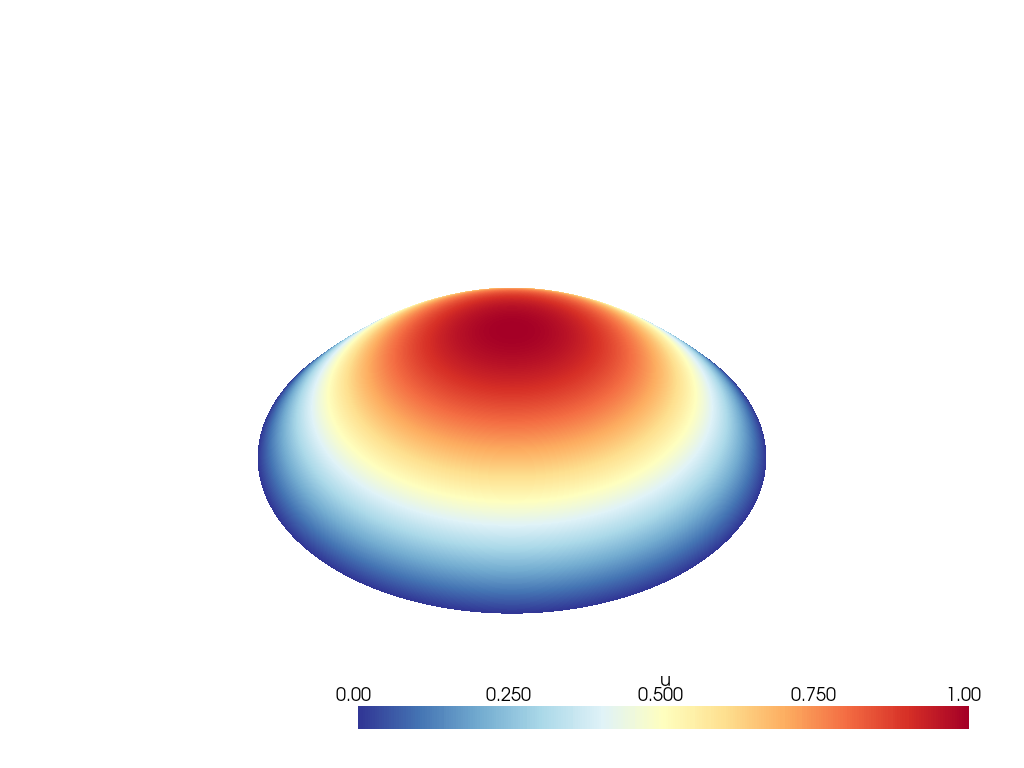
\includegraphics[width=0.5\textwidth,height=\textheight]{../img/mesh5-gauss02.png}
\caption{Finite element solution using order-2 Gaussian quadrature}
\end{figure}

\begin{quote}
What is the exact solution?
\end{quote}

The exact solution is

\[
\boxed{u = 1 - x^2 - y^2}
\]

\begin{figure}
\centering
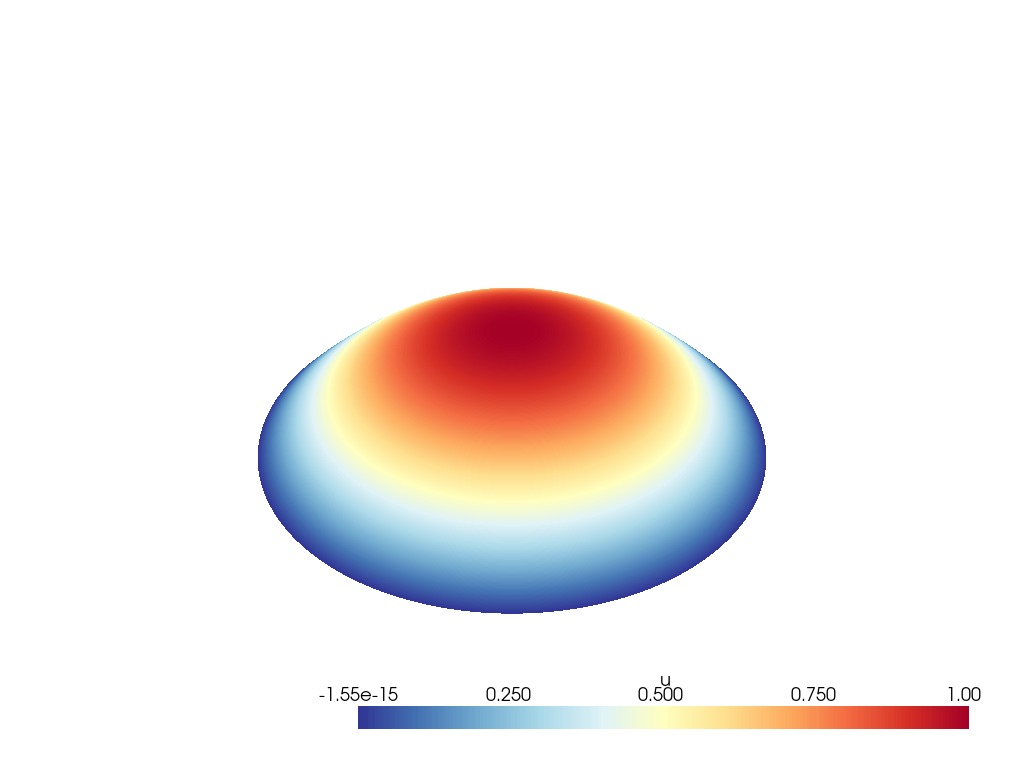
\includegraphics[width=0.5\textwidth,height=\textheight]{../img/analytic-a.png}
\caption{Closed-form solution to the stated Poisson problem.}
\end{figure}

\begin{quote}
Compute the \(H^1\) seminorm and \(L^2\) norm of the error for each of
the meshes. Ignore the fringe error due to the piecewise parabolic mesh
boundary not quite aligning with the circular domain.
\end{quote}

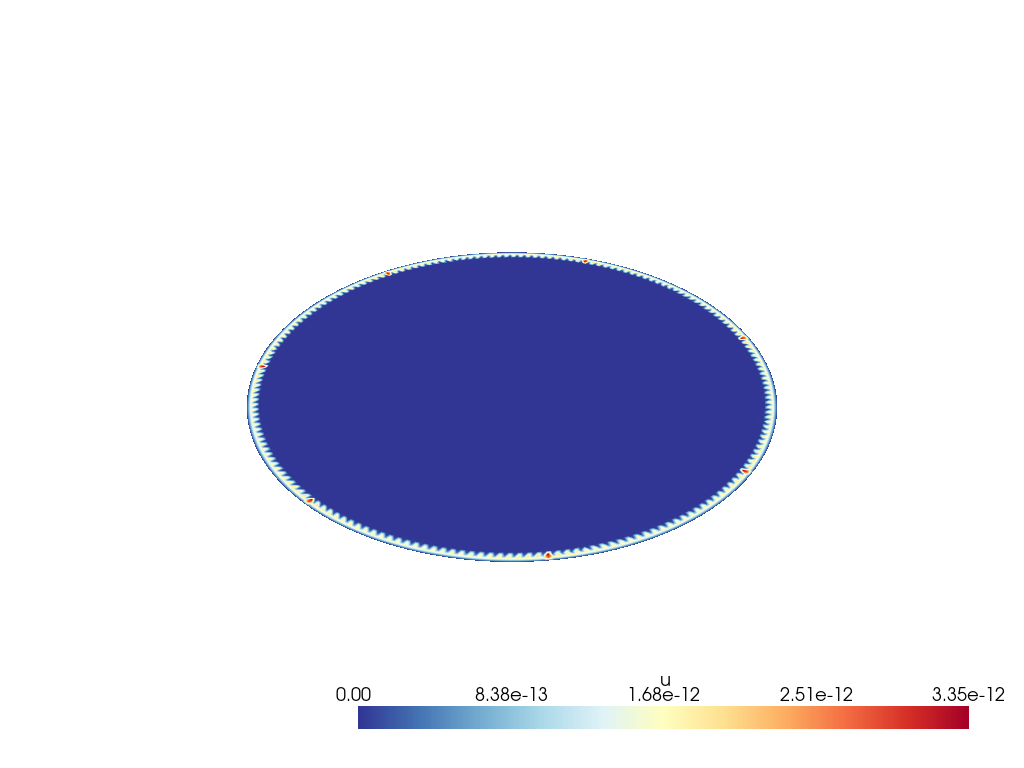
\includegraphics[width=0.5\textwidth,height=\textheight]{../img/mesh5-gauss02-H1.png}
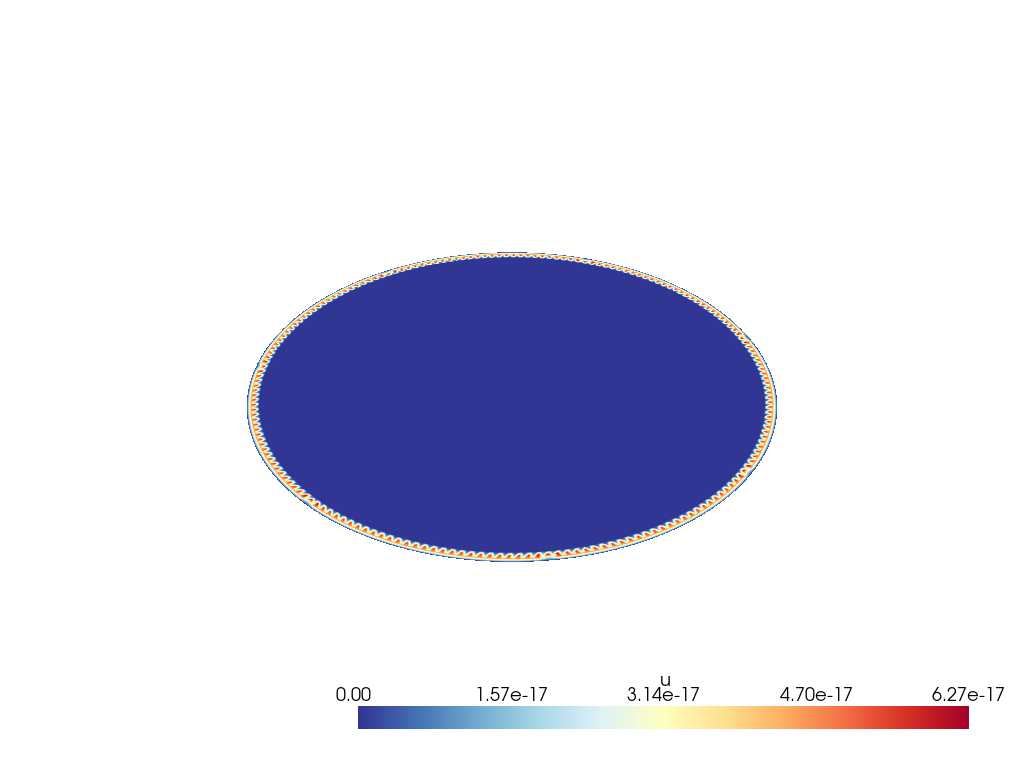
\includegraphics[width=0.5\textwidth,height=\textheight]{../img/mesh5-gauss02-L2.png}

\newpage{}

\begin{quote}
Turn in a table of your errors and \(\log\)-\(\log\) plots of the error
vs.\textasciitilde the mesh parameter, \(h\).
\end{quote}

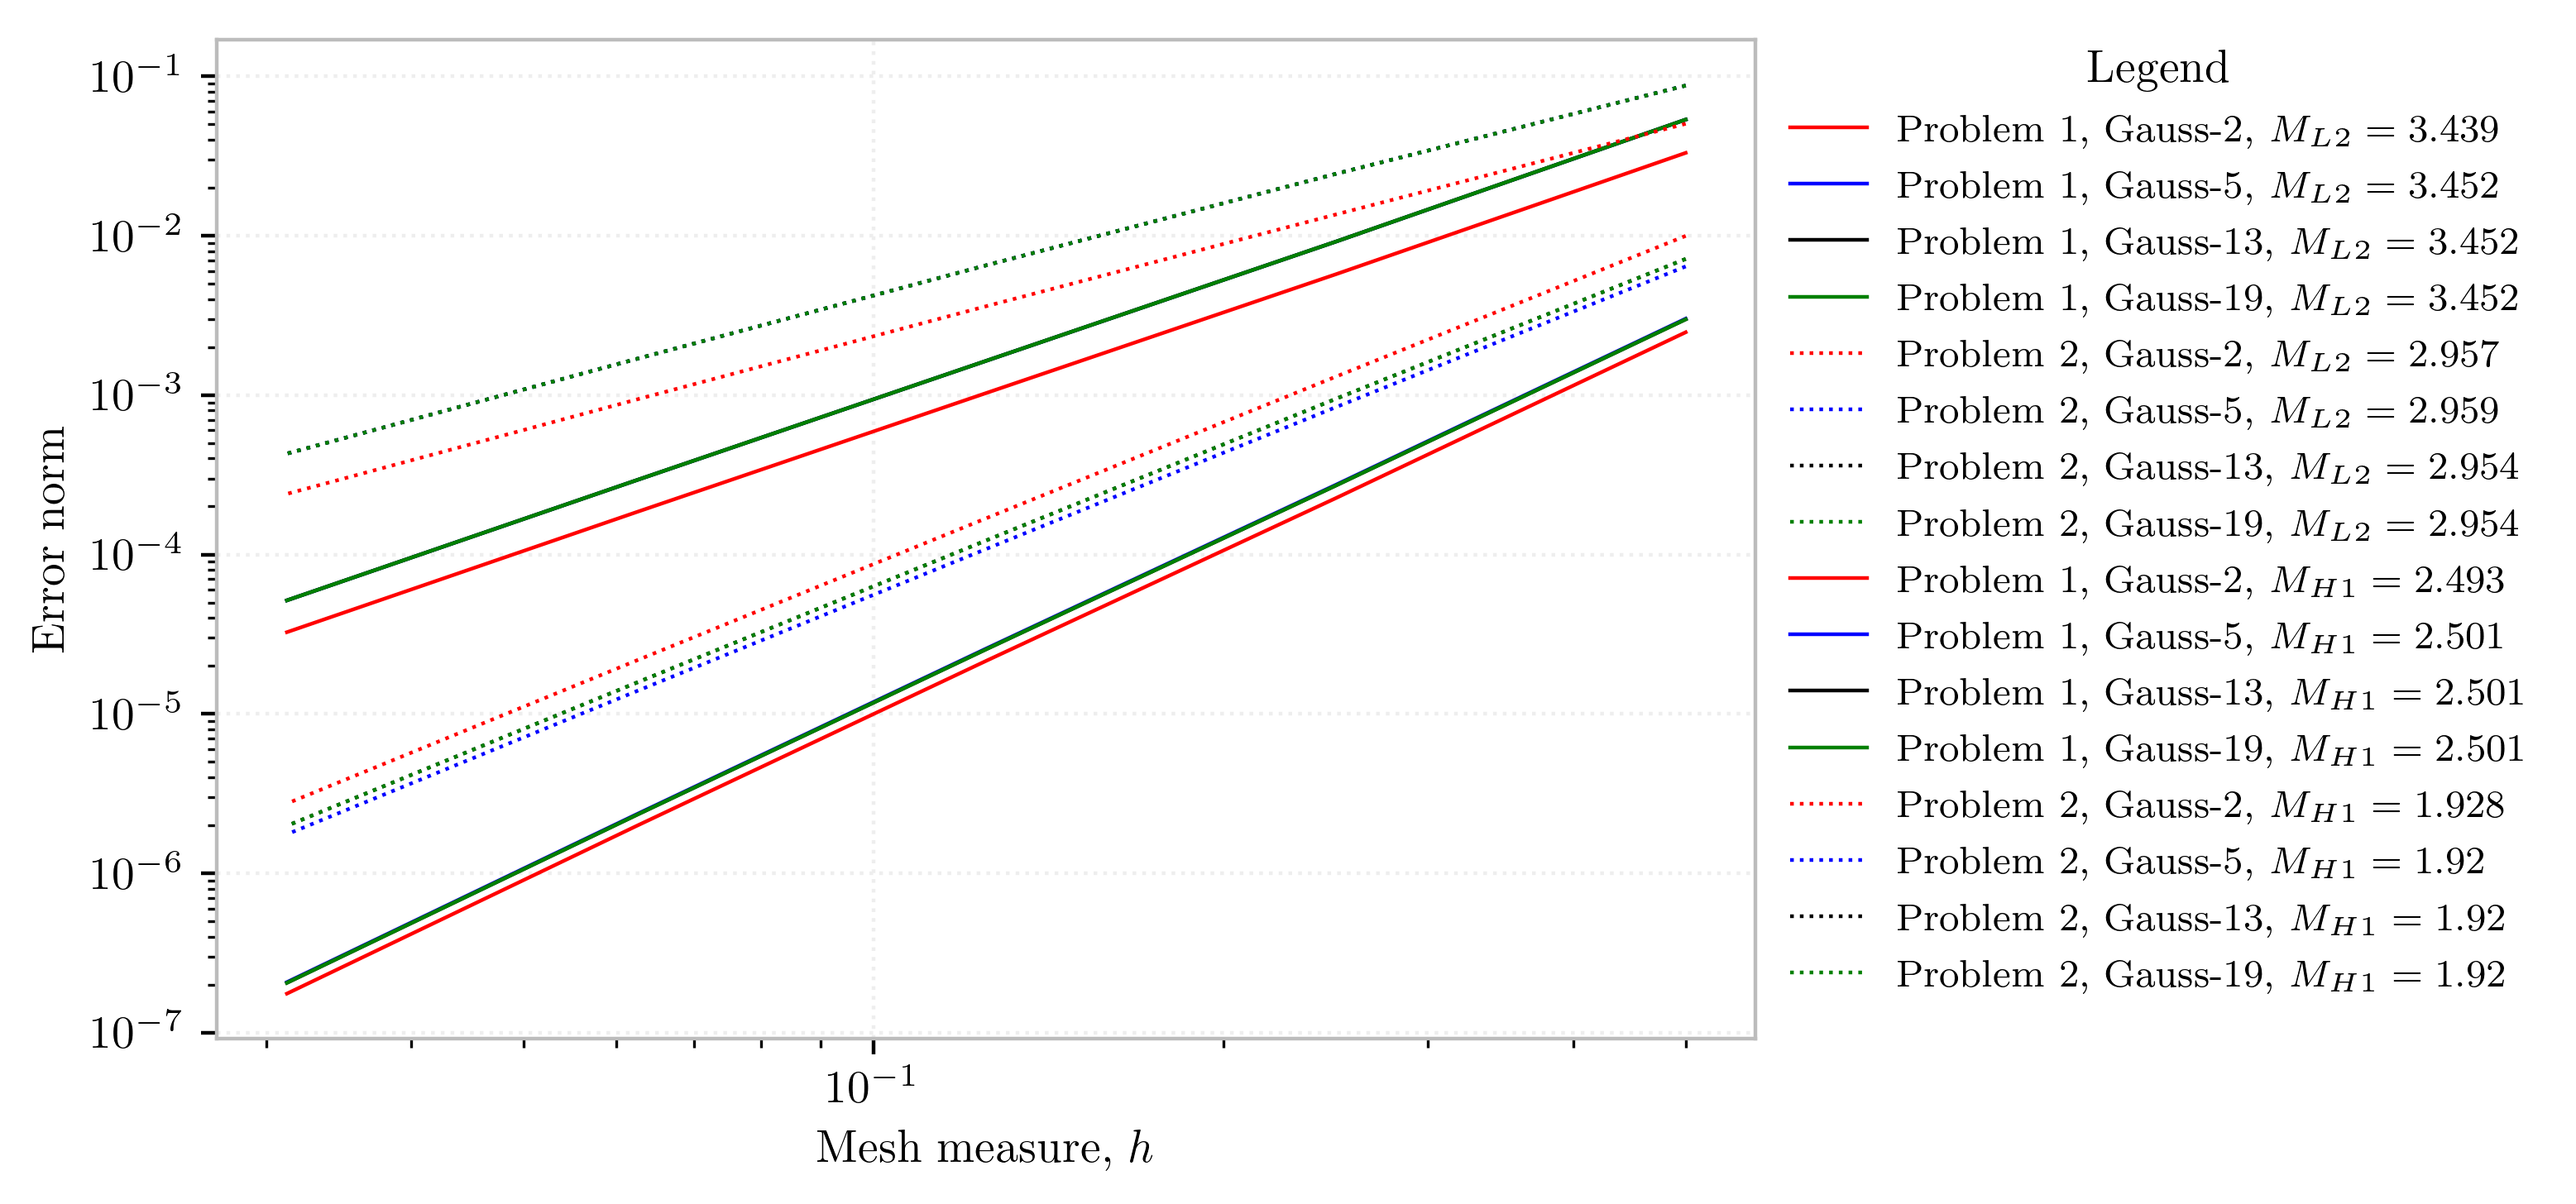
\includegraphics{../img/conv-3.png}

Table of errors in the L2 norm for problem 1

\begin{longtable}[]{@{}lllll@{}}
\toprule
\(h\) & 2 & 5 & 13 & 19 \\
\midrule
\endhead
0.5 & 0.0024764578 & 0.0030141854 & 0.0029849953 & 0.0029849953 \\
0.25 & 0.0002258162 & 0.00027375659 & 0.00027090969 & 0.00027090969 \\
0.125 & 2.1527457e-05 & 2.5708536e-05 & 2.5448945e-05 & 2.5448945e-05 \\
0.0625 & 1.9830323e-06 & 2.3460163e-06 & 2.3228069e-06 &
2.3228069e-06 \\
0.03125 & 1.7587735e-07 & 2.0760524e-07 & 2.0555351e-07 &
2.0555351e-07 \\
\bottomrule
\end{longtable}

Table of errors in the L2 norm for problem 2

\begin{longtable}[]{@{}lllll@{}}
\toprule
\(h\) & 2 & 5 & 13 & 19 \\
\midrule
\endhead
0.5 & 0.0099611923 & 0.0064076596 & 0.0071412137 & 0.0071412137 \\
0.25 & 0.0013051996 & 0.00083984741 & 0.0009471105 & 0.0009471105 \\
0.125 & 0.00016874334 & 0.00010830203 & 0.00012249798 & 0.00012249798 \\
0.0625 & 2.1626624e-05 & 1.3882073e-05 & 1.5691434e-05 &
1.5691434e-05 \\
0.03125 & 2.7380054e-06 & 1.756023e-06 & 1.9850051e-06 &
1.9850051e-06 \\
\bottomrule
\end{longtable}

Table of errors in the H1 norm for problem 1

\begin{longtable}[]{@{}lllll@{}}
\toprule
\(h\) & 2 & 5 & 13 & 19 \\
\midrule
\endhead
0.5 & 0.033040555 & 0.05344312 & 0.053451002 & 0.053451002 \\
0.25 & 0.0057268302 & 0.0091748492 & 0.0091751946 & 0.0091751946 \\
0.125 & 0.0010299012 & 0.0016399388 & 0.0016399544 & 0.0016399544 \\
0.0625 & 0.00018443725 & 0.00029237375 & 0.00029237444 &
0.00029237444 \\
0.03125 & 3.254096e-05 & 5.152993e-05 & 5.1529961e-05 & 5.1529961e-05 \\
\bottomrule
\end{longtable}

Table of errors in the H1 norm for problem 2

\begin{longtable}[]{@{}lllll@{}}
\toprule
\(h\) & 2 & 5 & 13 & 19 \\
\midrule
\endhead
0.5 & 0.050321736 & 0.087419539 & 0.087364004 & 0.087364004 \\
0.25 & 0.013576873 & 0.024424342 & 0.024421502 & 0.024421502 \\
0.125 & 0.0036081315 & 0.0065157661 & 0.006515551 & 0.006515551 \\
0.0625 & 0.00093741811 & 0.0016853971 & 0.0016853811 & 0.0016853811 \\
0.03125 & 0.00023986093 & 0.00042915864 & 0.00042915753 &
0.00042915753 \\
\bottomrule
\end{longtable}

\newpage{}

\hypertarget{problem-2}{%
\section{Problem 2}\label{problem-2}}

\begin{quote}
Repeat (1) for the problem

\[
 \begin{aligned}
   -\Delta u &= \frac{\pi^2}{4}\left(\cos\frac{\pi r}{2} +
   \operatorname{sinc} \frac{\pi r}{2}\right), & \quad &\text{in $\Omega$} \\
           u &= 0, & &\text{on $\partial\Omega$}
 \end{aligned}
\]

where \(\Omega\) is again the unit disk. The exact solution is
\(u(x,y)=\cos \frac{\pi r}{2}\), where \(r=\sqrt{x^2+y^2}\).
\end{quote}

\begin{figure}
\centering
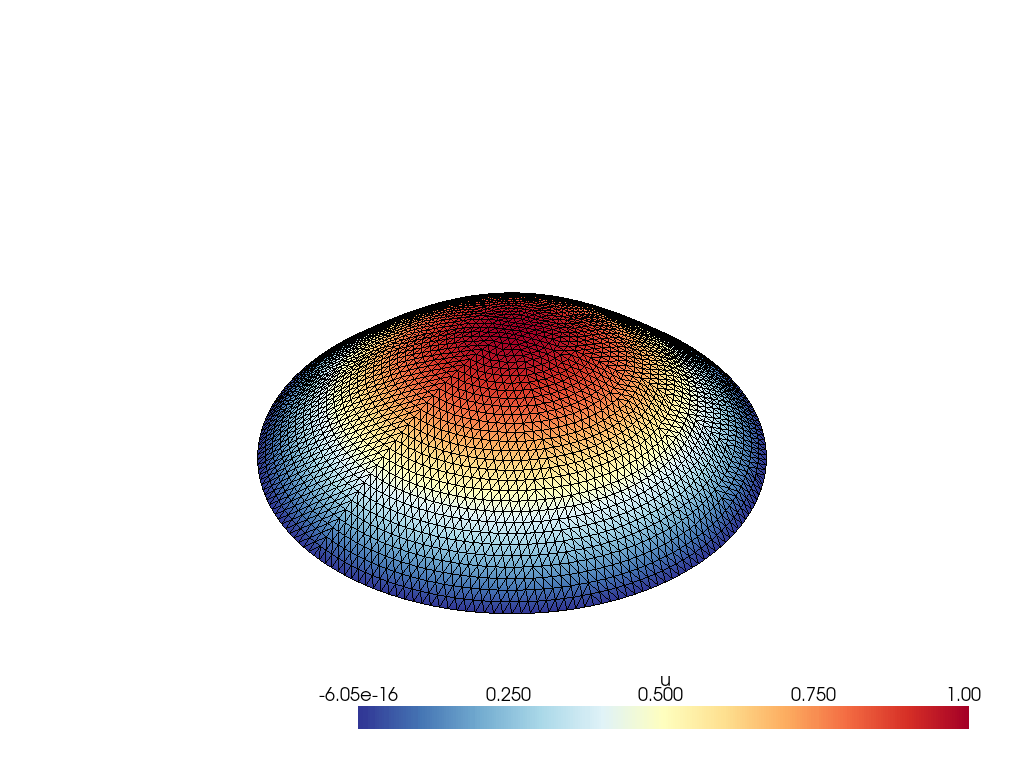
\includegraphics[width=0.5\textwidth,height=\textheight]{../img/analytic-b.png}
\caption{Plot of the given closed-form solution.}
\end{figure}

\newpage{}

\hypertarget{problem-3}{%
\section{Problem 3}\label{problem-3}}

\begin{quote}
(6 points) Explain why the convergence rate for problem (1) is half an
order higher than for problem (2). To understand what's going on, it may
be helpful to plot the contribution to the \(H^1\) and \(L^2\) errors
element by element. (see the sample file \texttt{plot\_errors.m}). For
example, in problem 2, I got the following values when I integrated

\[
\iint_T \nabla(u_{FE} - u_{exact}) \cdot
\nabla(u_{FE} - u_{exact})\,dx \, dy, \qquad
(T\in\mathcal{T})
\]

over the triangles in \texttt{circle\_iso/mesh3}:
\end{quote}

\begin{quote}
The \(H^1\) semi-norm error in the finite element solution is the square
root of the sum of all the errors shown here. (I got \(0.00400512\) for
the \(H^1\) error and \(7.5355\times10^{-5}\) for the \(L^2\) error on
this mesh).
\end{quote}

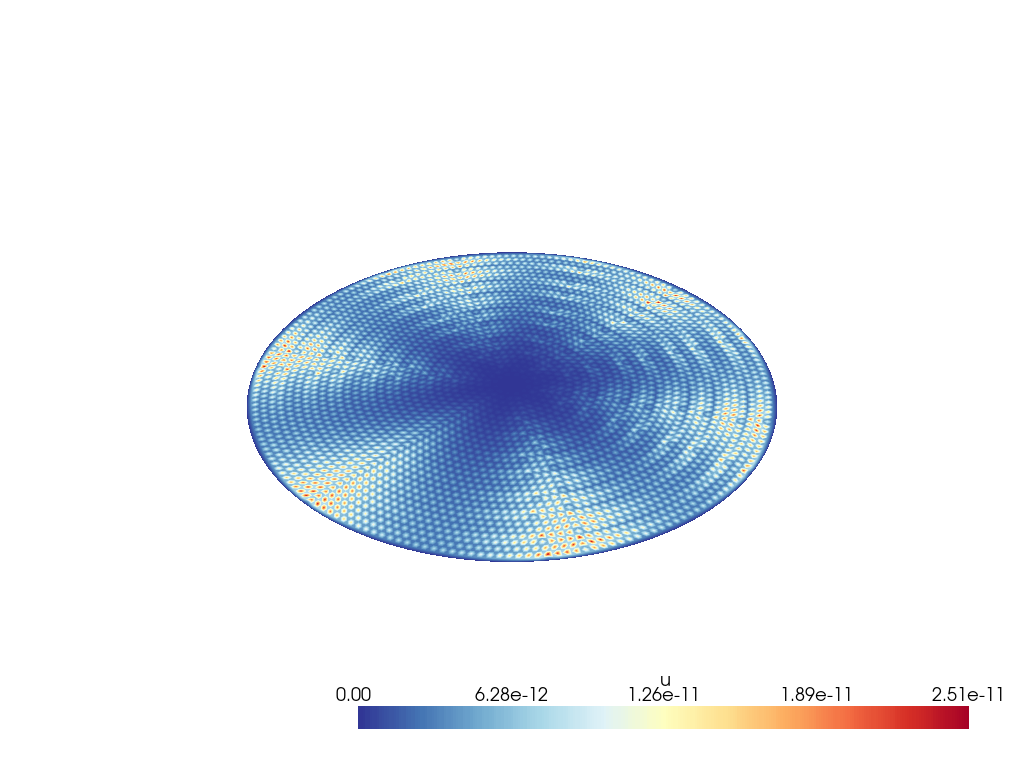
\includegraphics[width=0.5\textwidth,height=\textheight]{../img/mesh5-gauss02-b-H1.png}
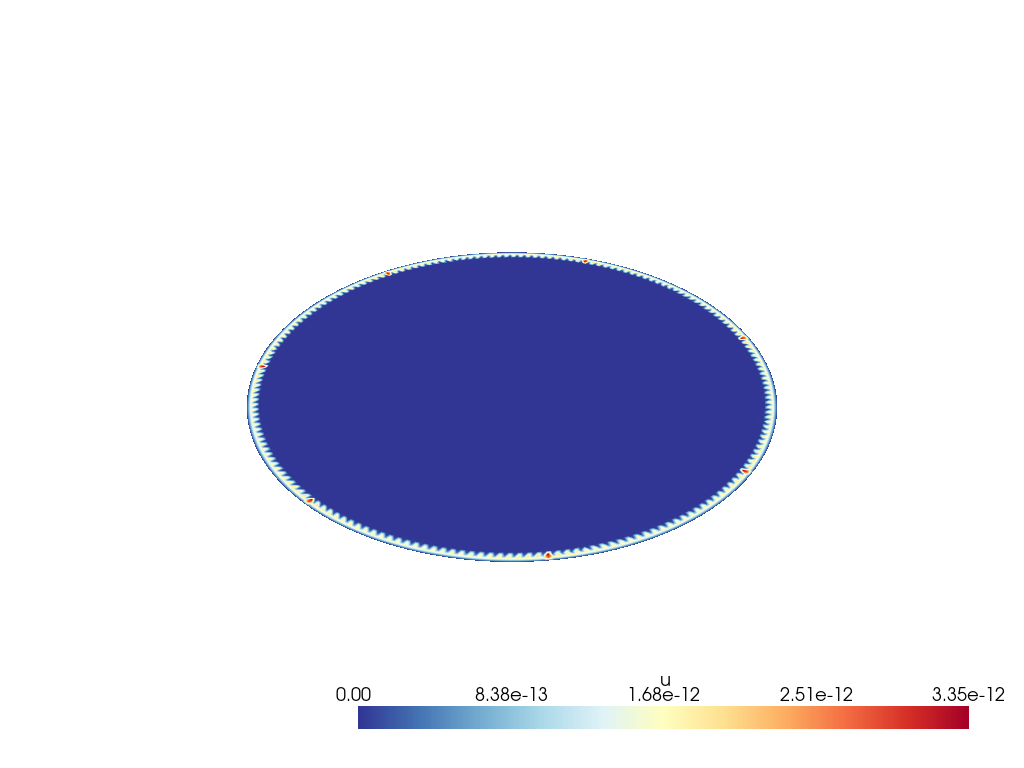
\includegraphics[width=0.5\textwidth,height=\textheight]{../img/mesh5-gauss02-H1.png}

\newpage{}

\hypertarget{appendix}{%
\section{Appendix}\label{appendix}}

\hypertarget{solution-plots}{%
\subsection{Solution plots}\label{solution-plots}}

\hypertarget{plots-of-finite-element-solutions}{%
\subsubsection{Plots of Finite Element
Solutions}\label{plots-of-finite-element-solutions}}

\begin{figure}
\centering
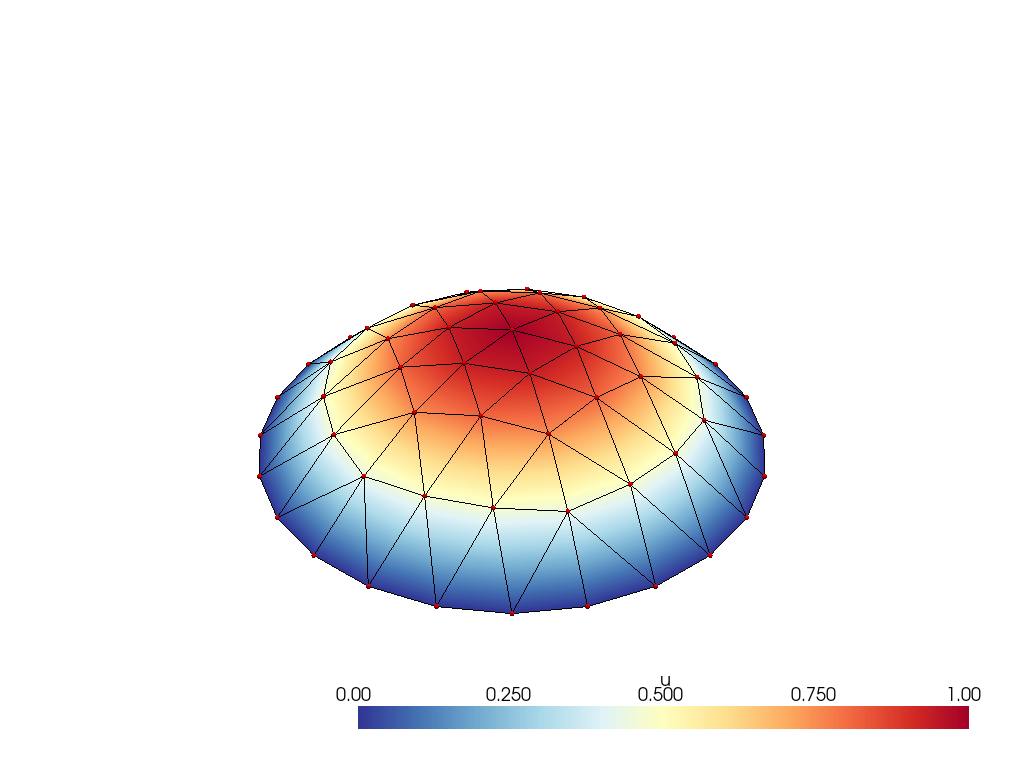
\includegraphics[width=0.5\textwidth,height=\textheight]{../img/mesh1-gauss02.png}
\caption{Finite element solution for problem 1 over mesh number 1 and
order-2 numerical integration.}
\end{figure}

\begin{figure}
\centering
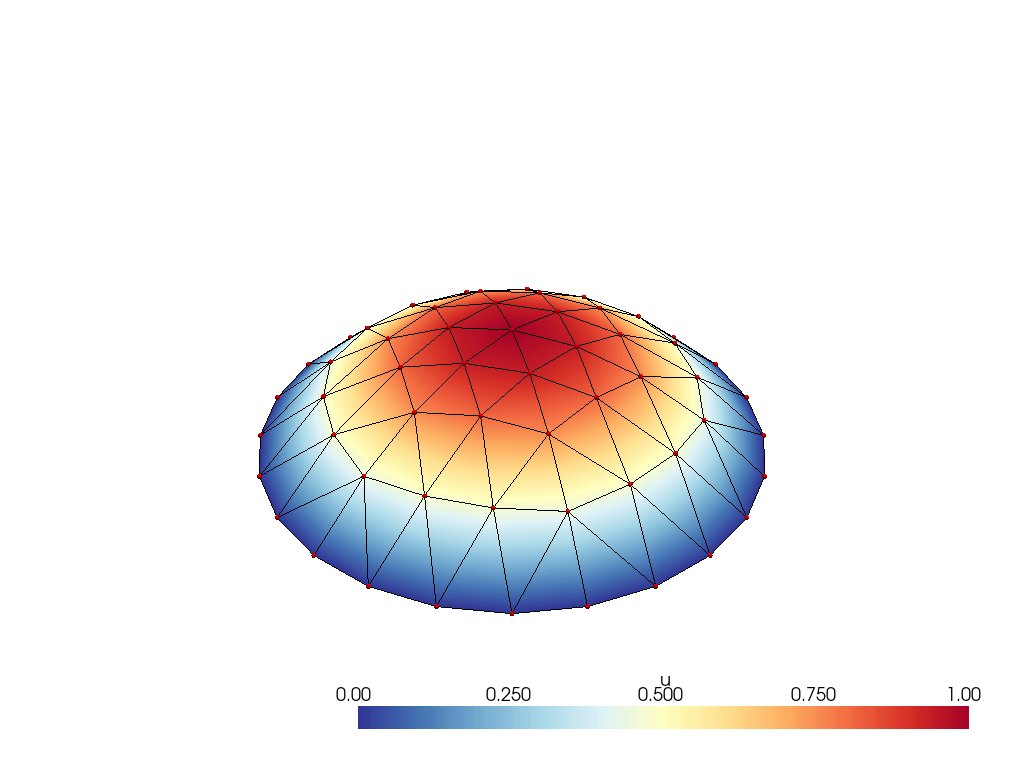
\includegraphics[width=0.5\textwidth,height=\textheight]{../img/mesh1-gauss05.png}
\caption{Finite element solution for problem 1 over mesh number 1 and
order-5 numerical integration.}
\end{figure}

\begin{figure}
\centering
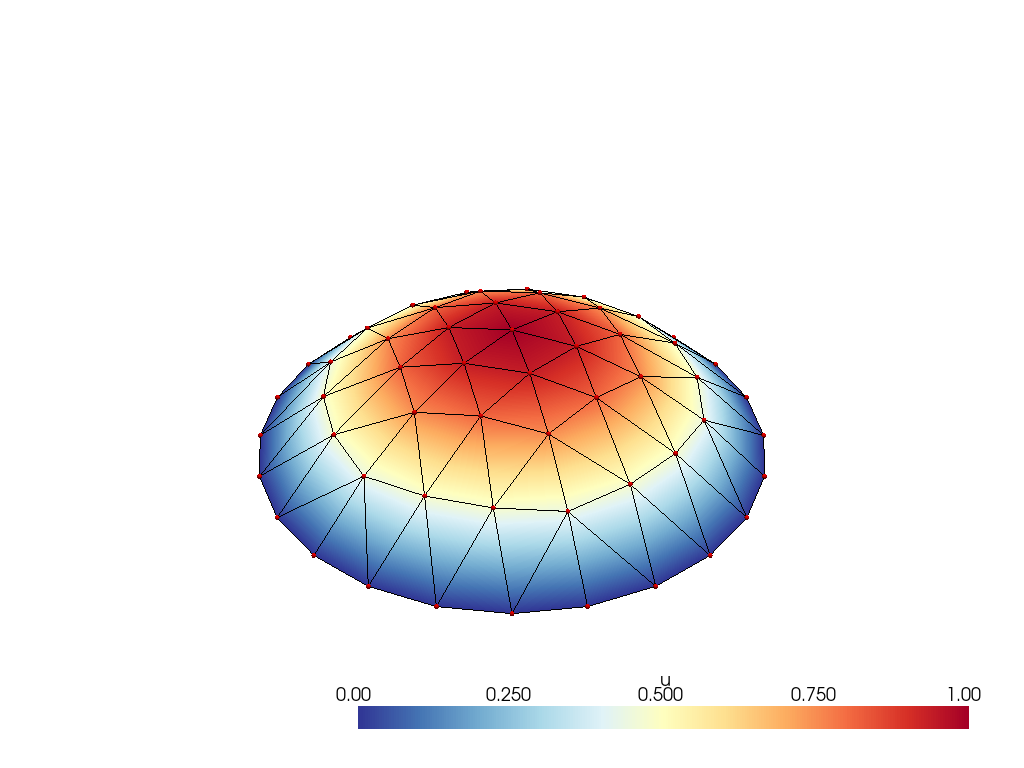
\includegraphics[width=0.5\textwidth,height=\textheight]{../img/mesh1-gauss08.png}
\caption{Finite element solution for problem 1 over mesh number 1 and
order-8 numerical integration.}
\end{figure}

\begin{figure}
\centering
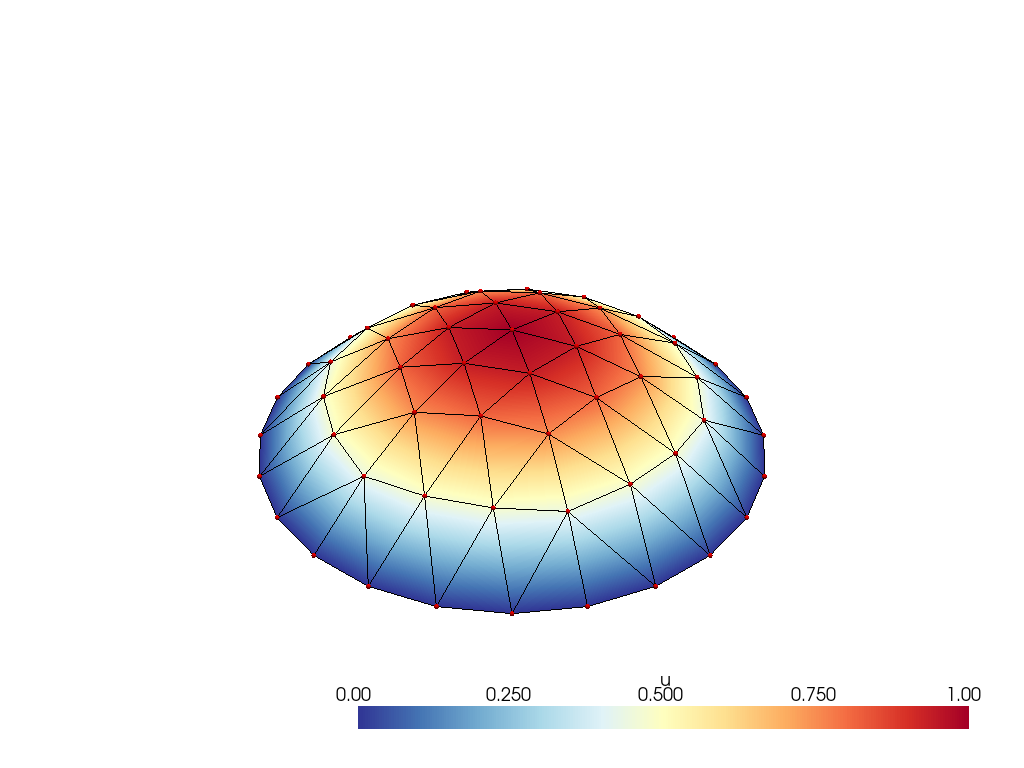
\includegraphics[width=0.5\textwidth,height=\textheight]{../img/mesh1-gauss13.png}
\caption{Finite element solution for problem 1 over mesh number 1 and
order-13 numerical integration.}
\end{figure}

\begin{figure}
\centering
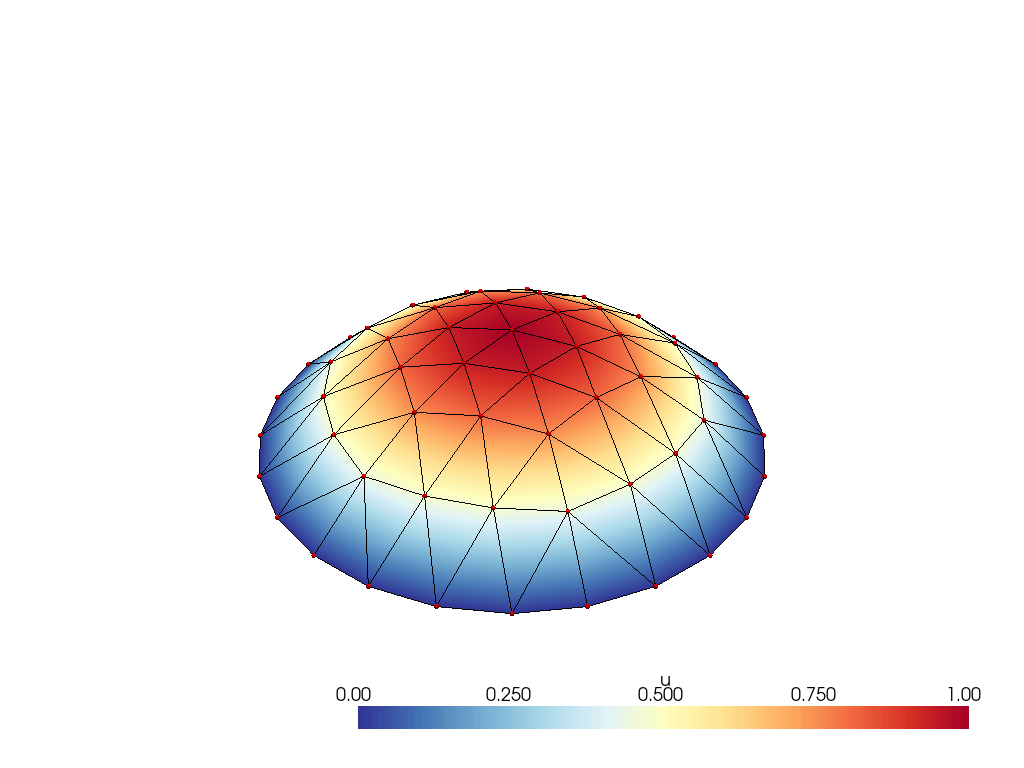
\includegraphics[width=0.5\textwidth,height=\textheight]{../img/mesh1-gauss19.png}
\caption{Finite element solution for problem 1 over mesh number 1 and
order-19 numerical integration.}
\end{figure}

\begin{figure}
\centering
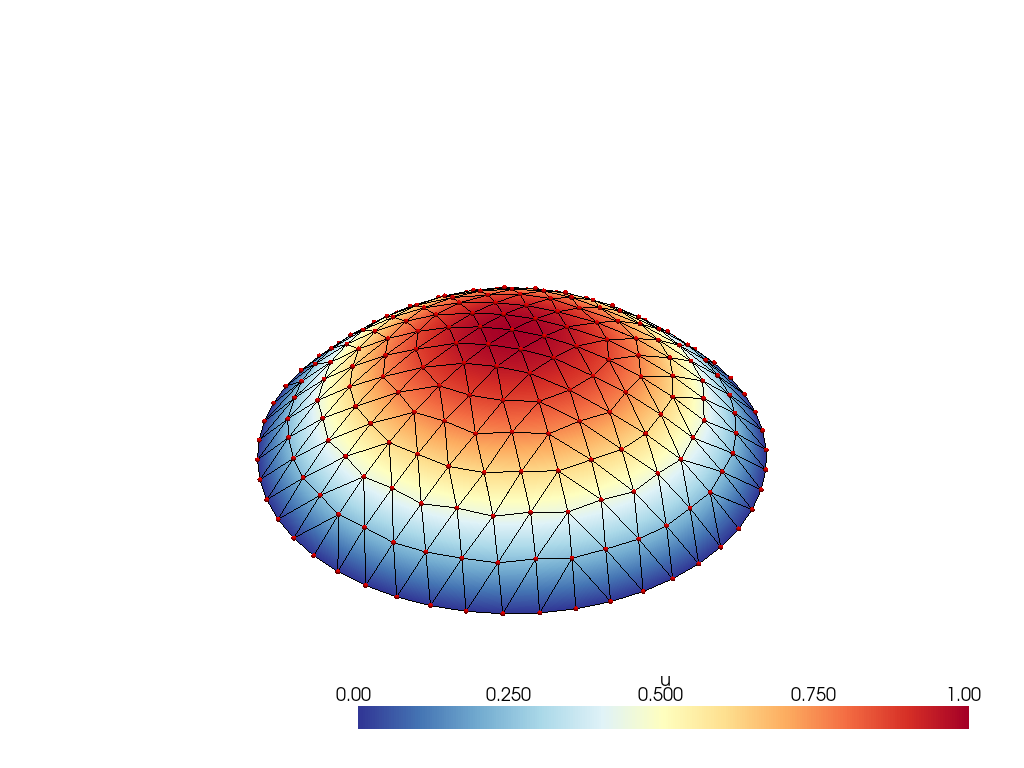
\includegraphics[width=0.5\textwidth,height=\textheight]{../img/mesh2-gauss02.png}
\caption{Finite element solution for problem 1 over mesh number 2 and
order-2 numerical integration.}
\end{figure}

\begin{figure}
\centering
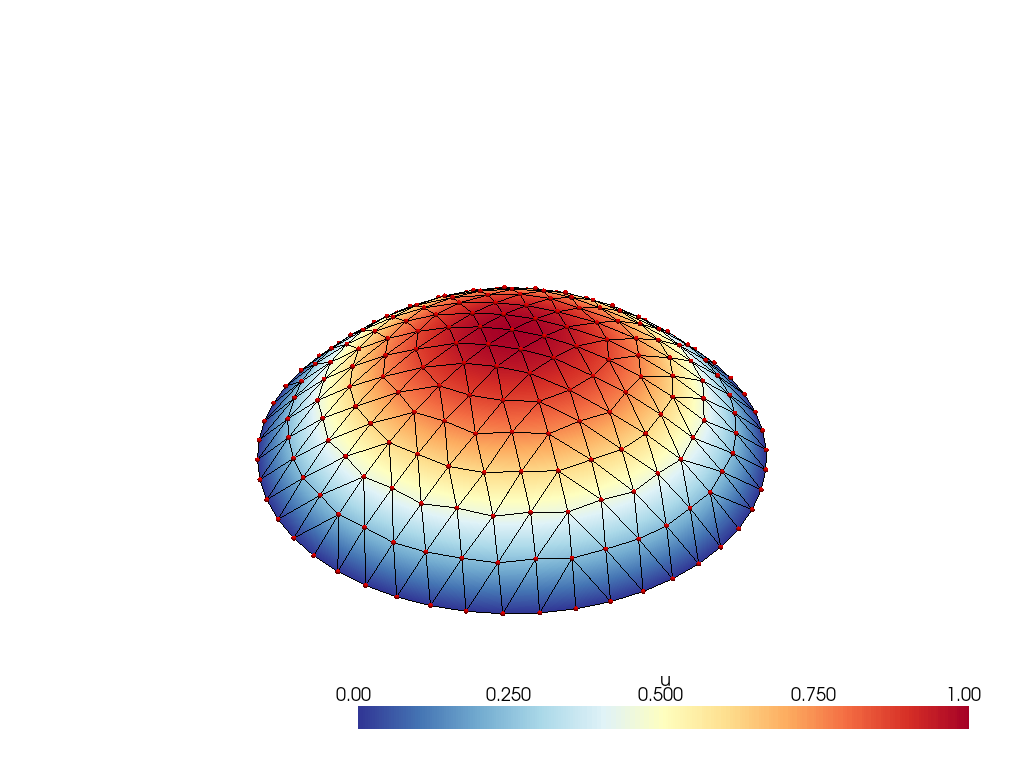
\includegraphics[width=0.5\textwidth,height=\textheight]{../img/mesh2-gauss05.png}
\caption{Finite element solution for problem 1 over mesh number 2 and
order-5 numerical integration.}
\end{figure}

\begin{figure}
\centering
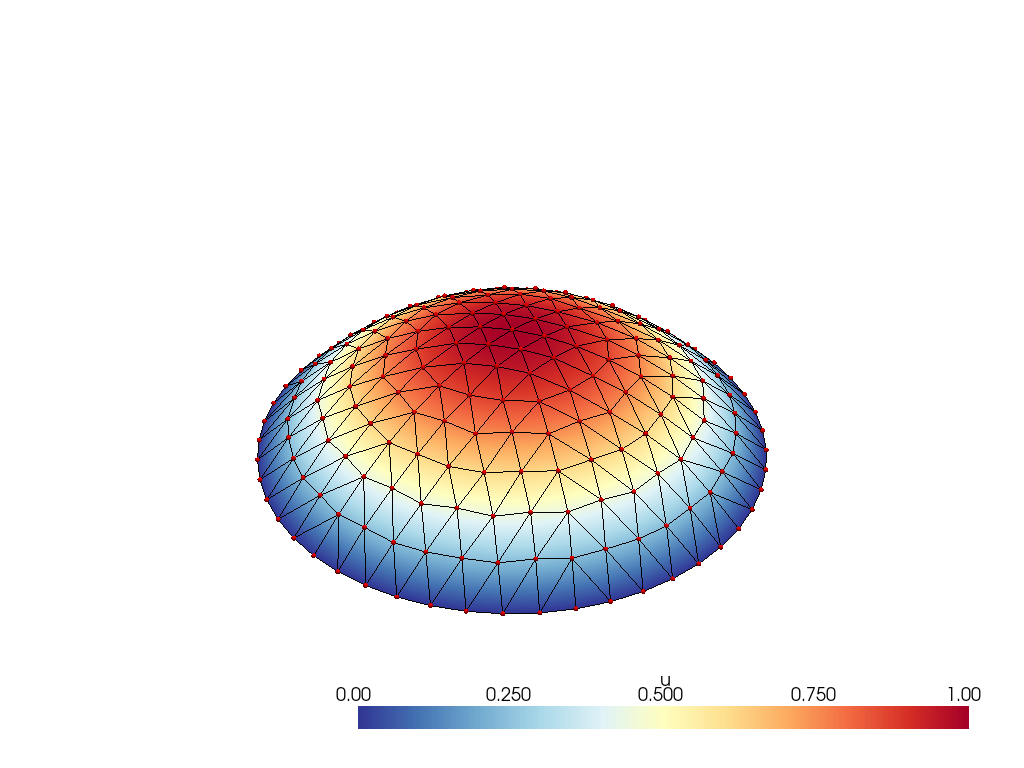
\includegraphics[width=0.5\textwidth,height=\textheight]{../img/mesh2-gauss08.png}
\caption{Finite element solution for problem 1 over mesh number 2 and
order-8 numerical integration.}
\end{figure}

\begin{figure}
\centering
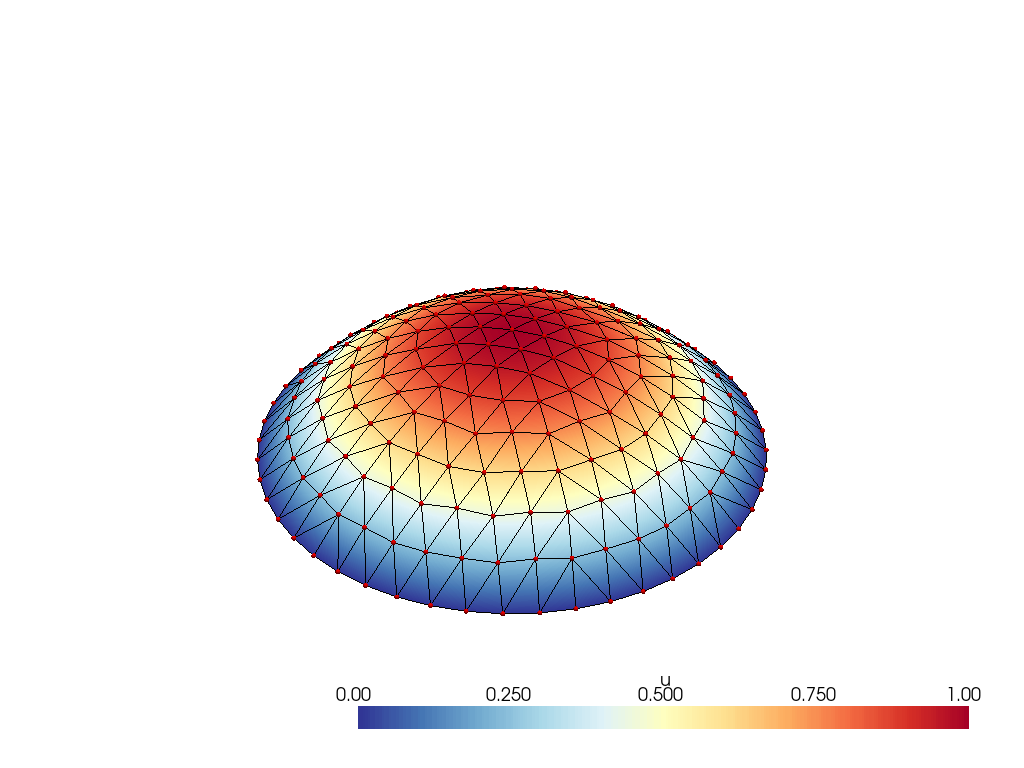
\includegraphics[width=0.5\textwidth,height=\textheight]{../img/mesh2-gauss13.png}
\caption{Finite element solution for problem 1 over mesh number 2 and
order-13 numerical integration.}
\end{figure}

\begin{figure}
\centering
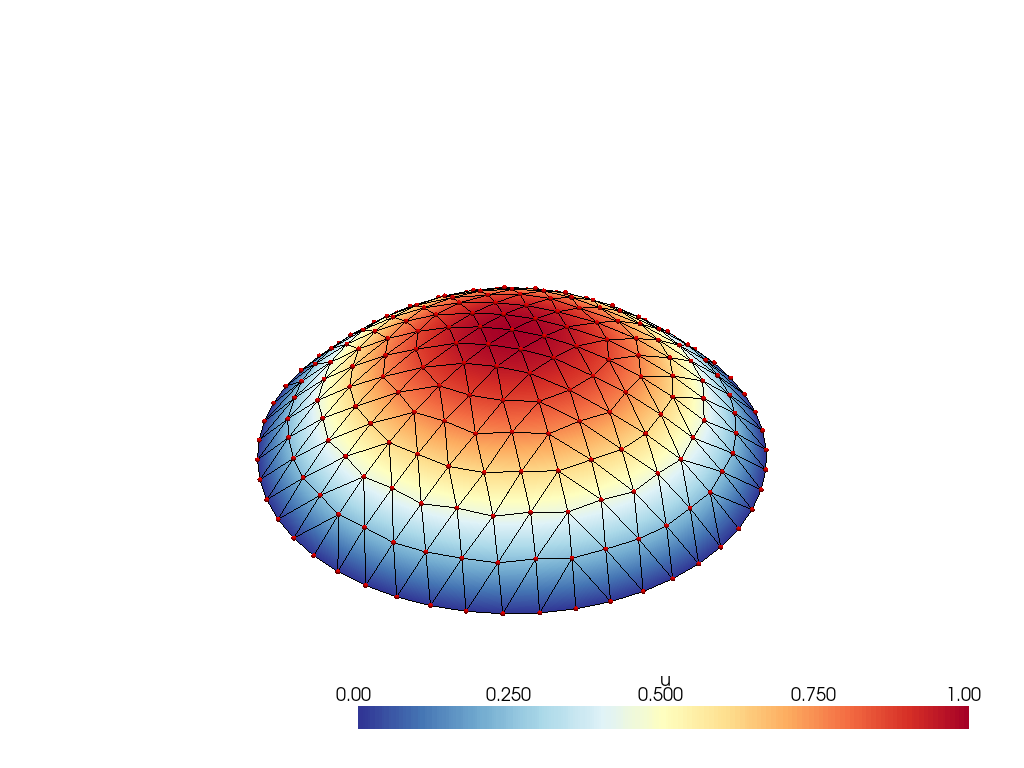
\includegraphics[width=0.5\textwidth,height=\textheight]{../img/mesh2-gauss19.png}
\caption{Finite element solution for problem 1 over mesh number 2 and
order-19 numerical integration.}
\end{figure}

\begin{figure}
\centering
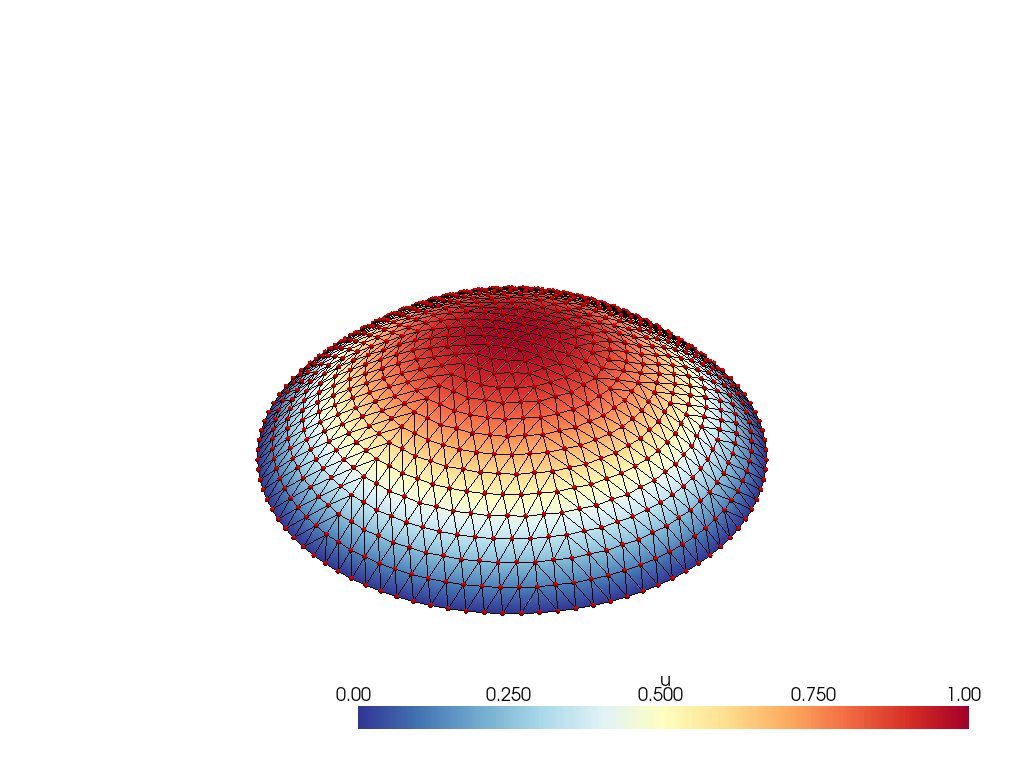
\includegraphics[width=0.5\textwidth,height=\textheight]{../img/mesh3-gauss02.png}
\caption{Finite element solution for problem 1 over mesh number 3 and
order-2 numerical integration.}
\end{figure}

\begin{figure}
\centering
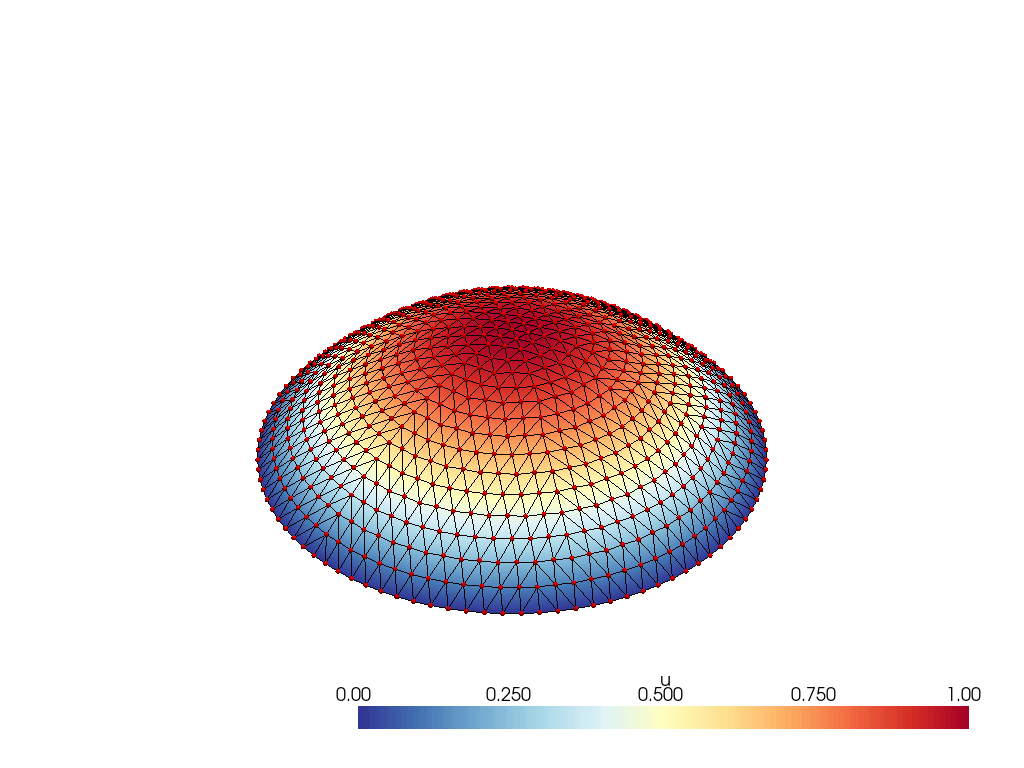
\includegraphics[width=0.5\textwidth,height=\textheight]{../img/mesh3-gauss05.png}
\caption{Finite element solution for problem 1 over mesh number 3 and
order-5 numerical integration.}
\end{figure}

\begin{figure}
\centering
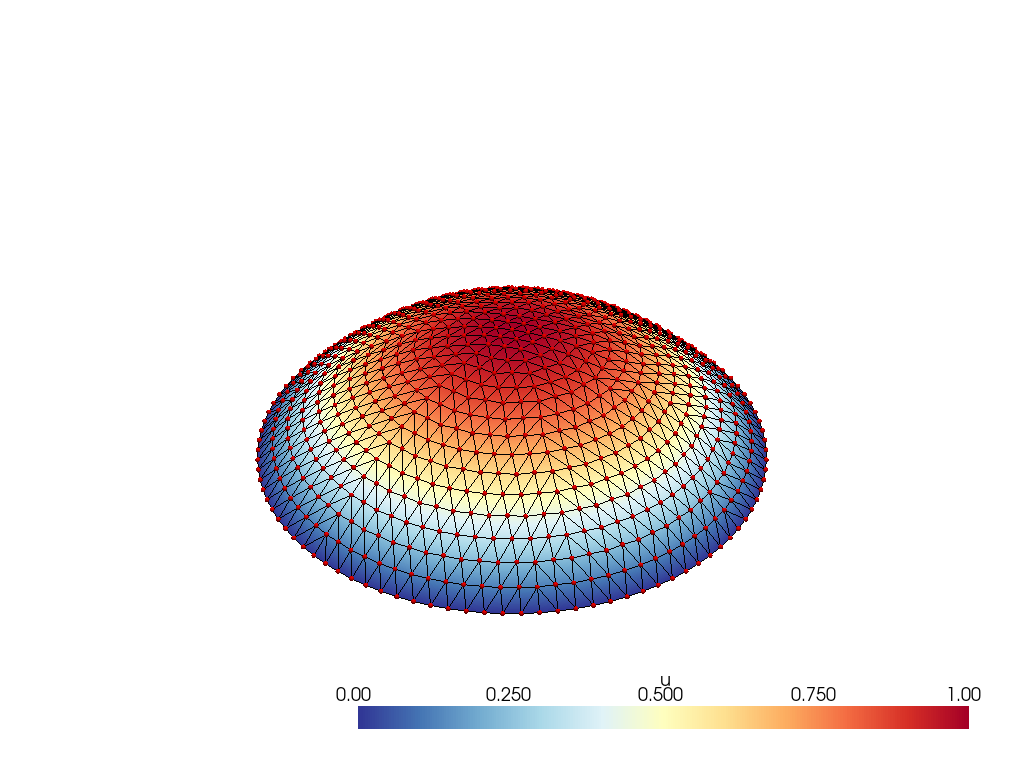
\includegraphics[width=0.5\textwidth,height=\textheight]{../img/mesh3-gauss08.png}
\caption{Finite element solution for problem 1 over mesh number 3 and
order-8 numerical integration.}
\end{figure}

\begin{figure}
\centering
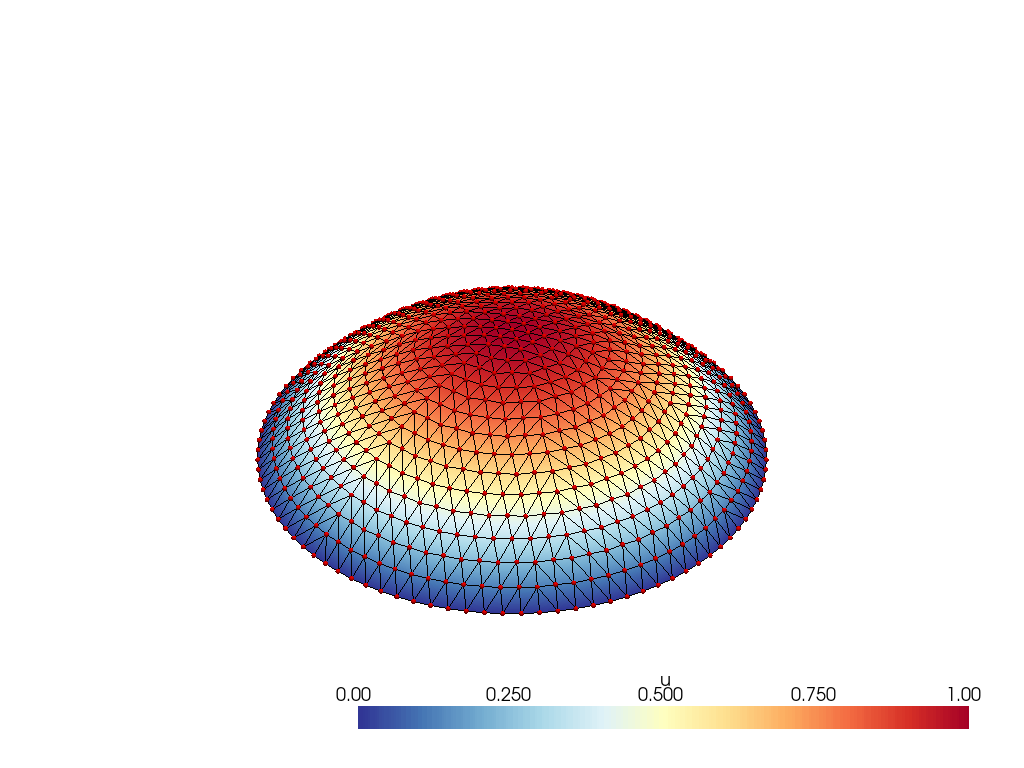
\includegraphics[width=0.5\textwidth,height=\textheight]{../img/mesh3-gauss13.png}
\caption{Finite element solution for problem 1 over mesh number 3 and
order-13 numerical integration.}
\end{figure}

\begin{figure}
\centering
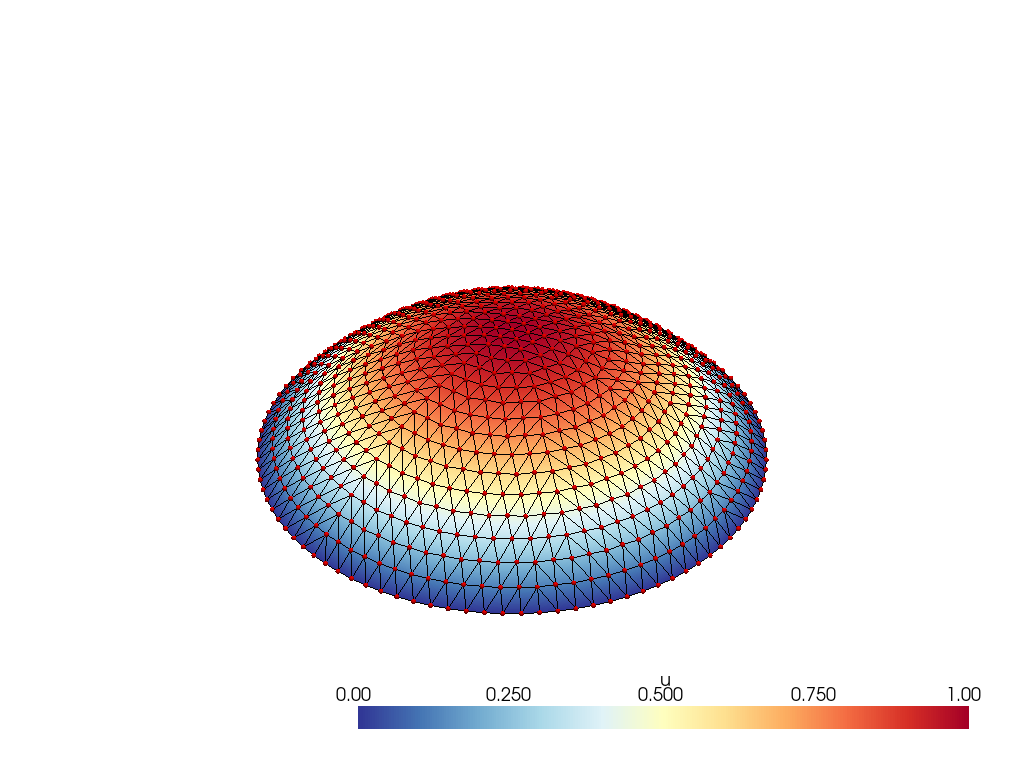
\includegraphics[width=0.5\textwidth,height=\textheight]{../img/mesh3-gauss19.png}
\caption{Finite element solution for problem 1 over mesh number 3 and
order-19 numerical integration.}
\end{figure}

\begin{figure}
\centering
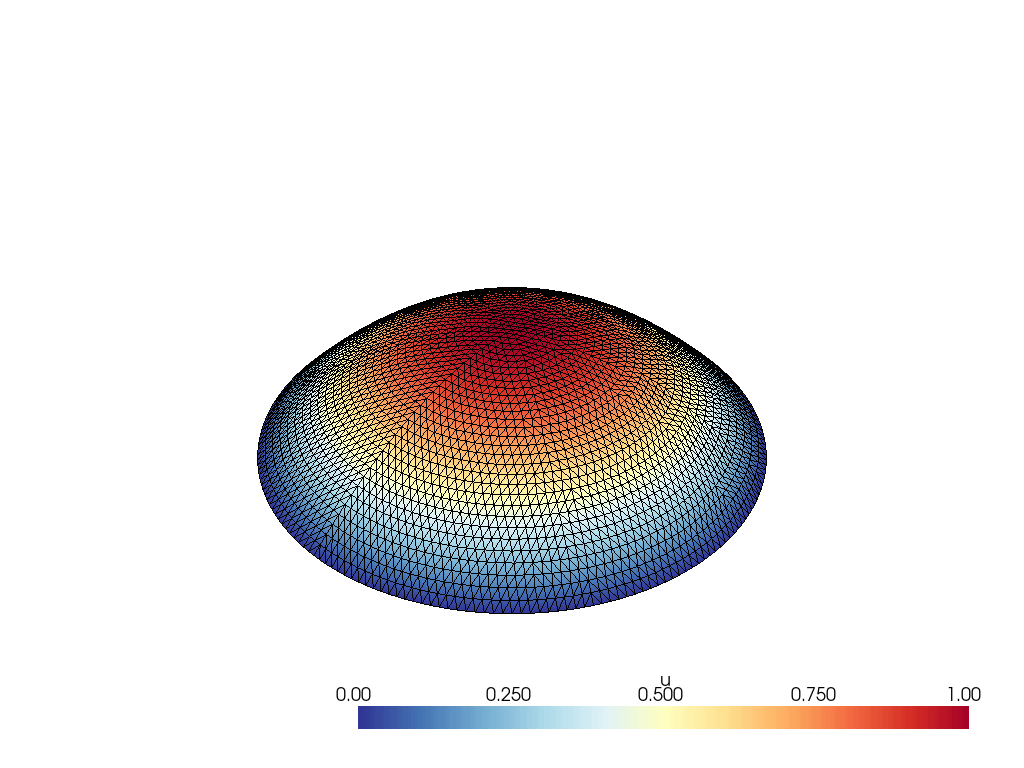
\includegraphics[width=0.5\textwidth,height=\textheight]{../img/mesh4-gauss02.png}
\caption{Finite element solution for problem 1 over mesh number 4 and
order-2 numerical integration.}
\end{figure}

\begin{figure}
\centering
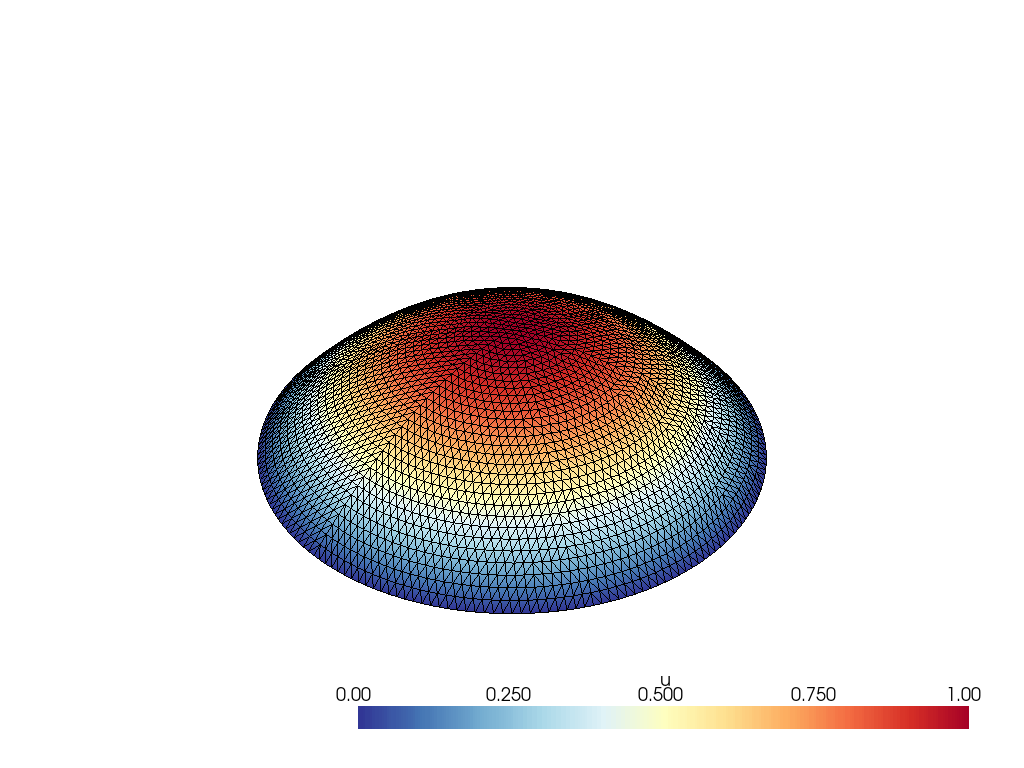
\includegraphics[width=0.5\textwidth,height=\textheight]{../img/mesh4-gauss05.png}
\caption{Finite element solution for problem 1 over mesh number 4 and
order-5 numerical integration.}
\end{figure}

\begin{figure}
\centering
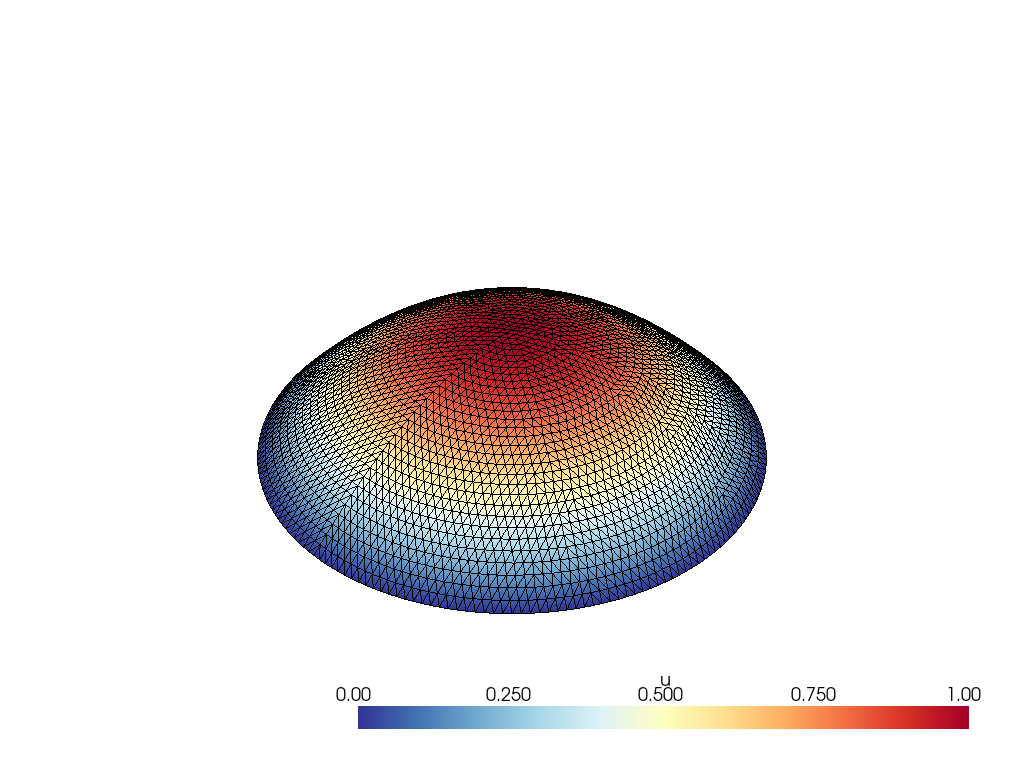
\includegraphics[width=0.5\textwidth,height=\textheight]{../img/mesh4-gauss08.png}
\caption{Finite element solution for problem 1 over mesh number 4 and
order-8 numerical integration.}
\end{figure}

\begin{figure}
\centering
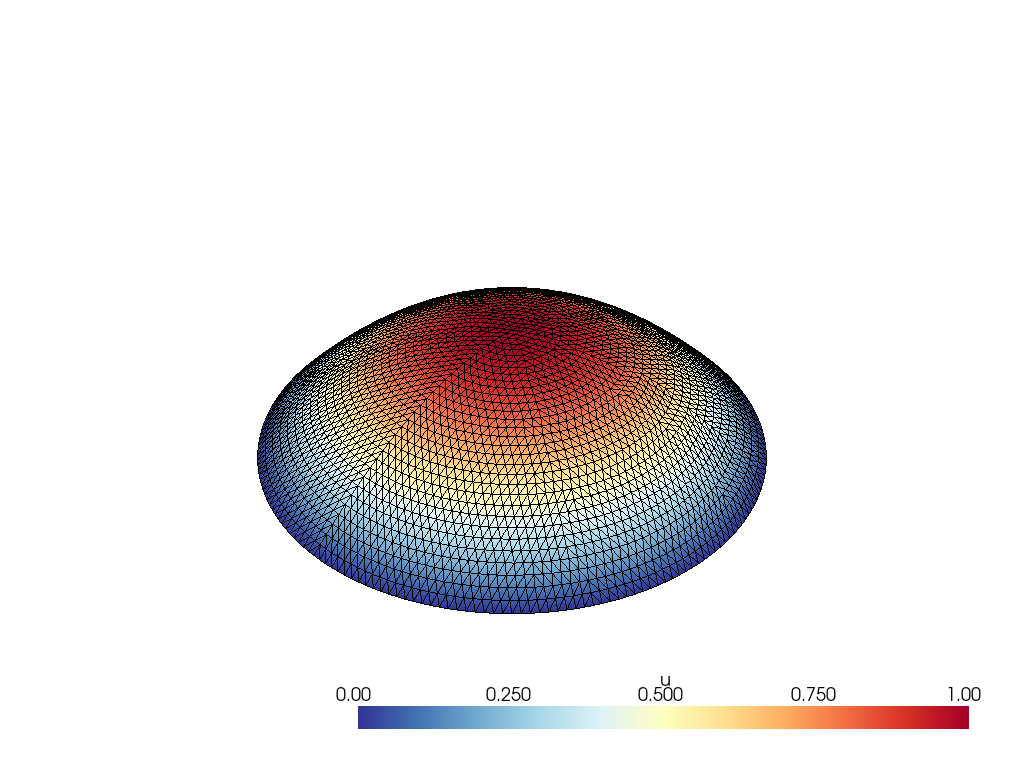
\includegraphics[width=0.5\textwidth,height=\textheight]{../img/mesh4-gauss13.png}
\caption{Finite element solution for problem 1 over mesh number 4 and
order-13 numerical integration.}
\end{figure}

\begin{figure}
\centering
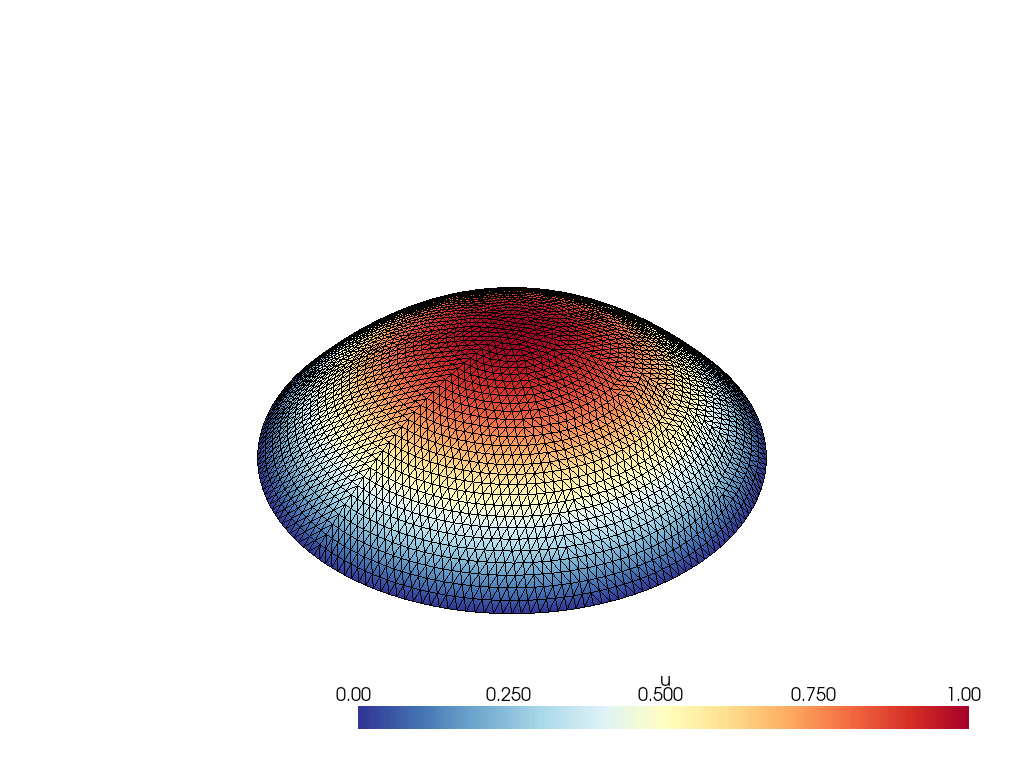
\includegraphics[width=0.5\textwidth,height=\textheight]{../img/mesh4-gauss19.png}
\caption{Finite element solution for problem 1 over mesh number 4 and
order-19 numerical integration.}
\end{figure}

\begin{figure}
\centering
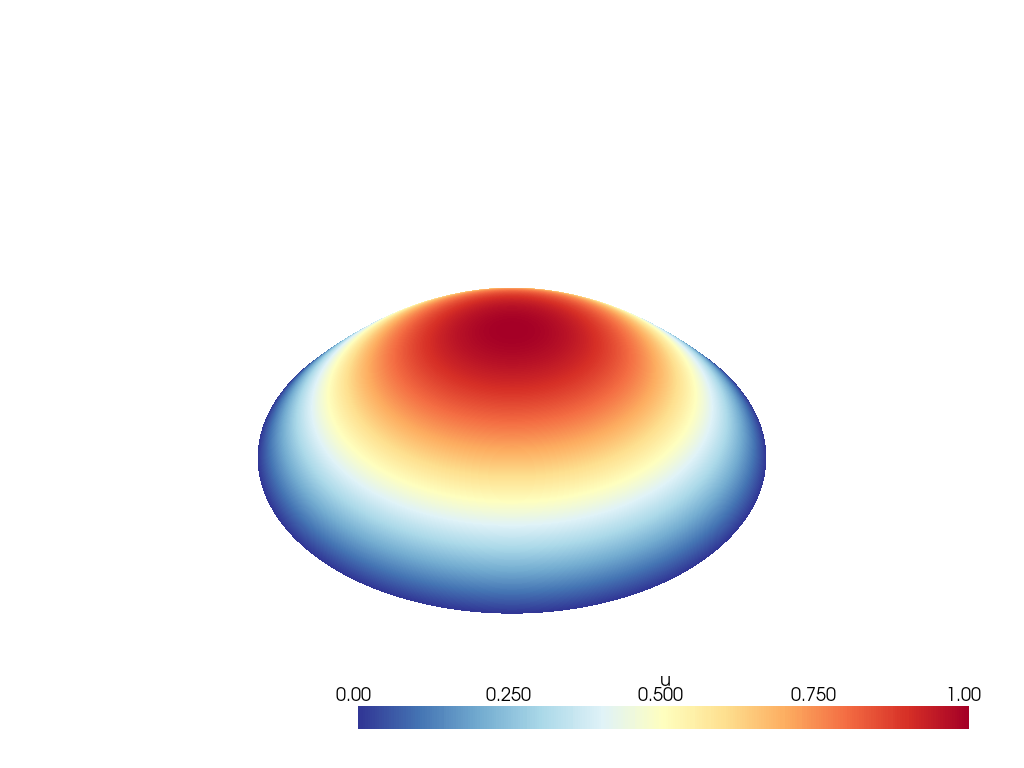
\includegraphics[width=0.5\textwidth,height=\textheight]{../img/mesh5-gauss02.png}
\caption{Finite element solution for problem 1 over mesh number 5 and
order-2 numerical integration.}
\end{figure}

\begin{figure}
\centering
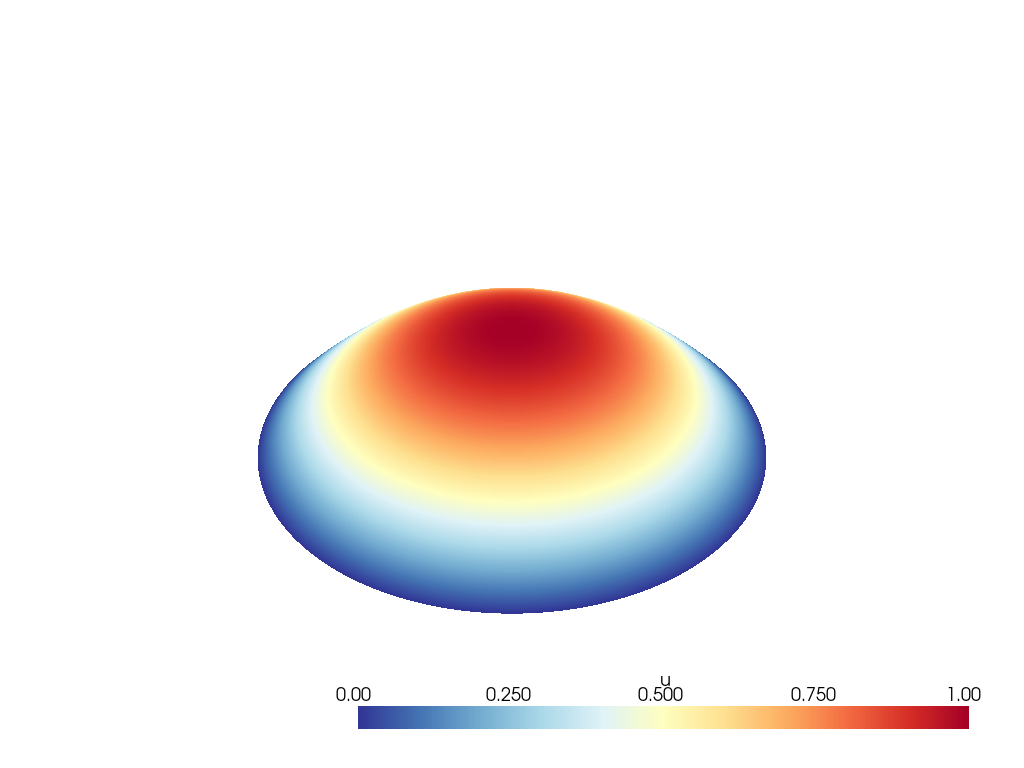
\includegraphics[width=0.5\textwidth,height=\textheight]{../img/mesh5-gauss05.png}
\caption{Finite element solution for problem 1 over mesh number 5 and
order-5 numerical integration.}
\end{figure}

\begin{figure}
\centering
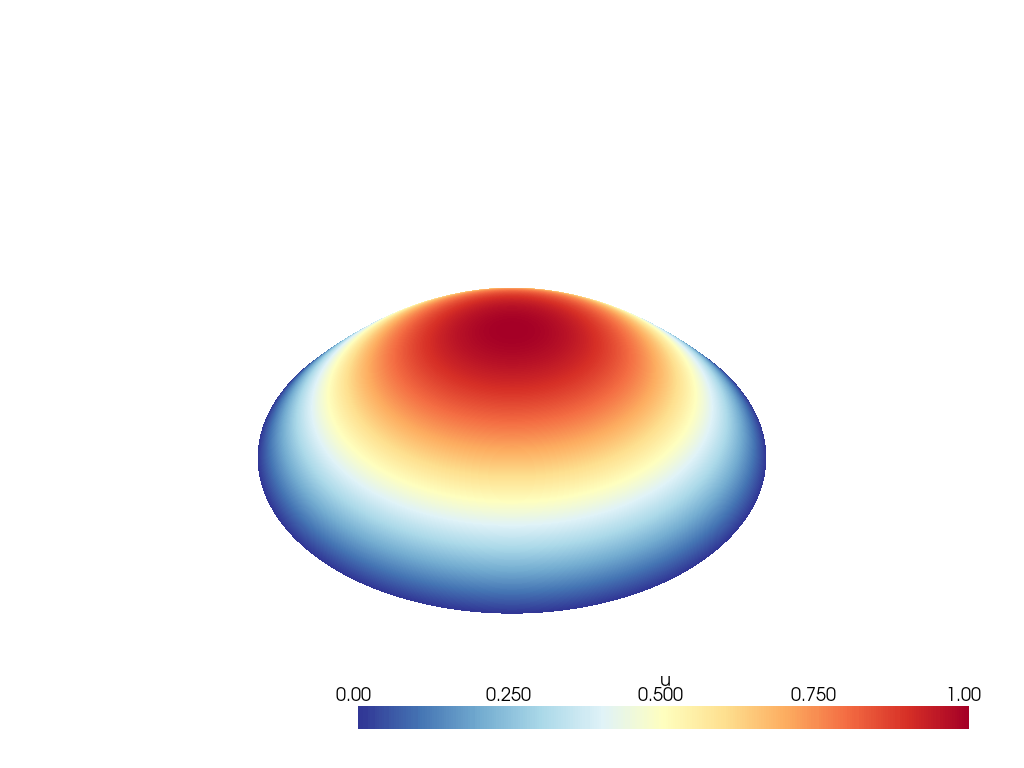
\includegraphics[width=0.5\textwidth,height=\textheight]{../img/mesh5-gauss08.png}
\caption{Finite element solution for problem 1 over mesh number 5 and
order-8 numerical integration.}
\end{figure}

\begin{figure}
\centering
\includegraphics[width=0.5\textwidth,height=\textheight]{../img/mesh5-gauss13.png}
\caption{Finite element solution for problem 1 over mesh number 5 and
order-13 numerical integration.}
\end{figure}

\begin{figure}
\centering
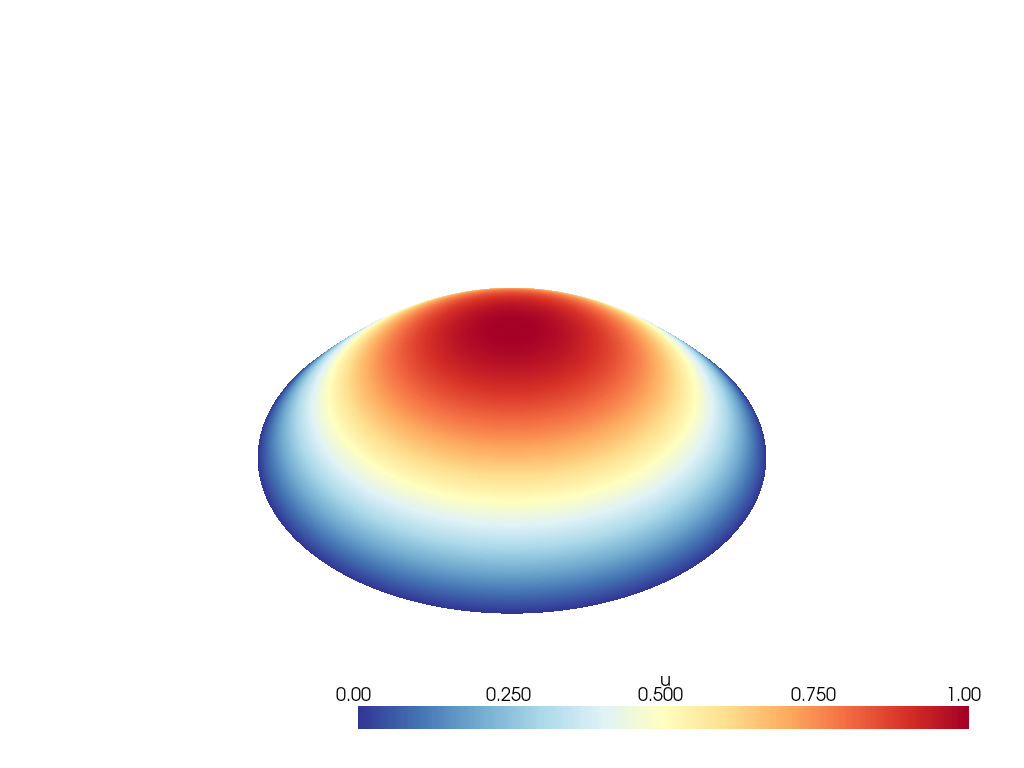
\includegraphics[width=0.5\textwidth,height=\textheight]{../img/mesh5-gauss19.png}
\caption{Finite element solution for problem 1 over mesh number 5 and
order-19 numerical integration.}
\end{figure}

\begin{figure}
\centering
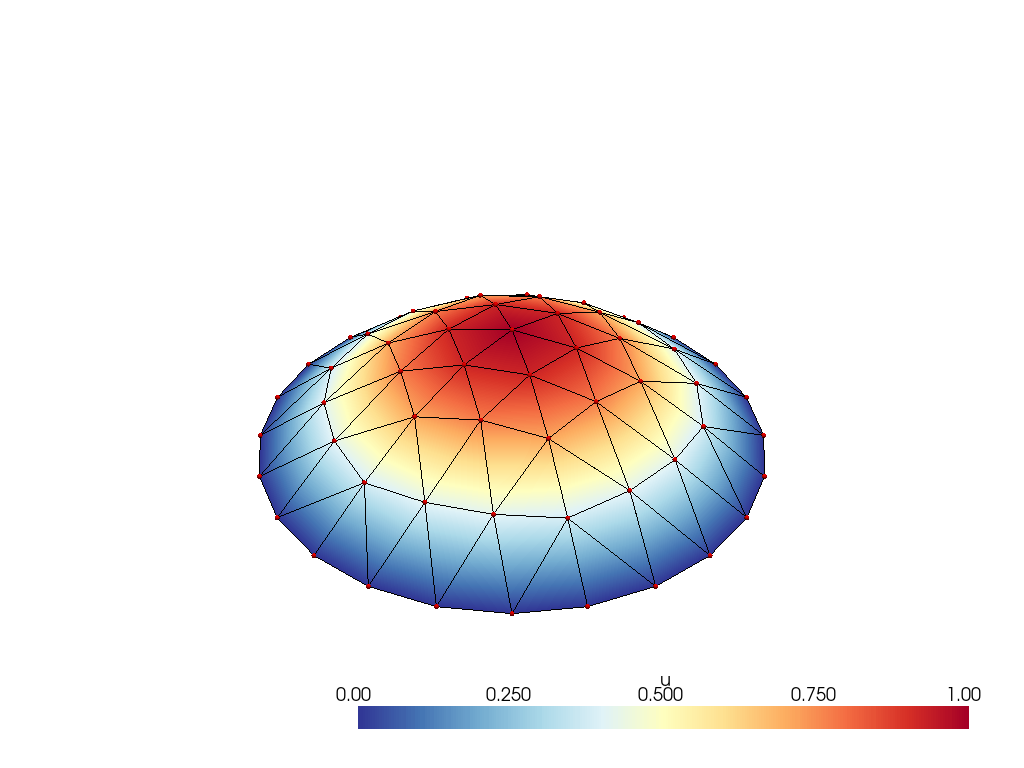
\includegraphics[width=0.5\textwidth,height=\textheight]{../img/mesh1-gauss02-b.png}
\caption{Finite element solution for problem 1 over mesh number 1 and
order-2 numerical integration.}
\end{figure}

\begin{figure}
\centering
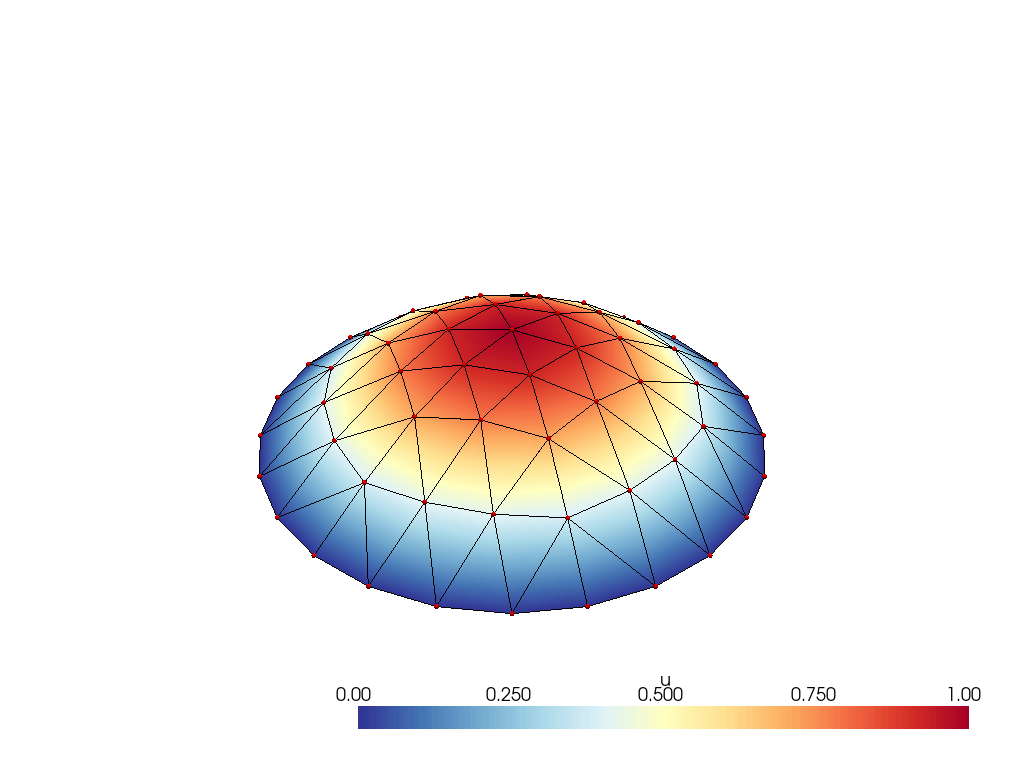
\includegraphics[width=0.5\textwidth,height=\textheight]{../img/mesh1-gauss05-b.png}
\caption{Finite element solution for problem 1 over mesh number 1 and
order-5 numerical integration.}
\end{figure}

\begin{figure}
\centering
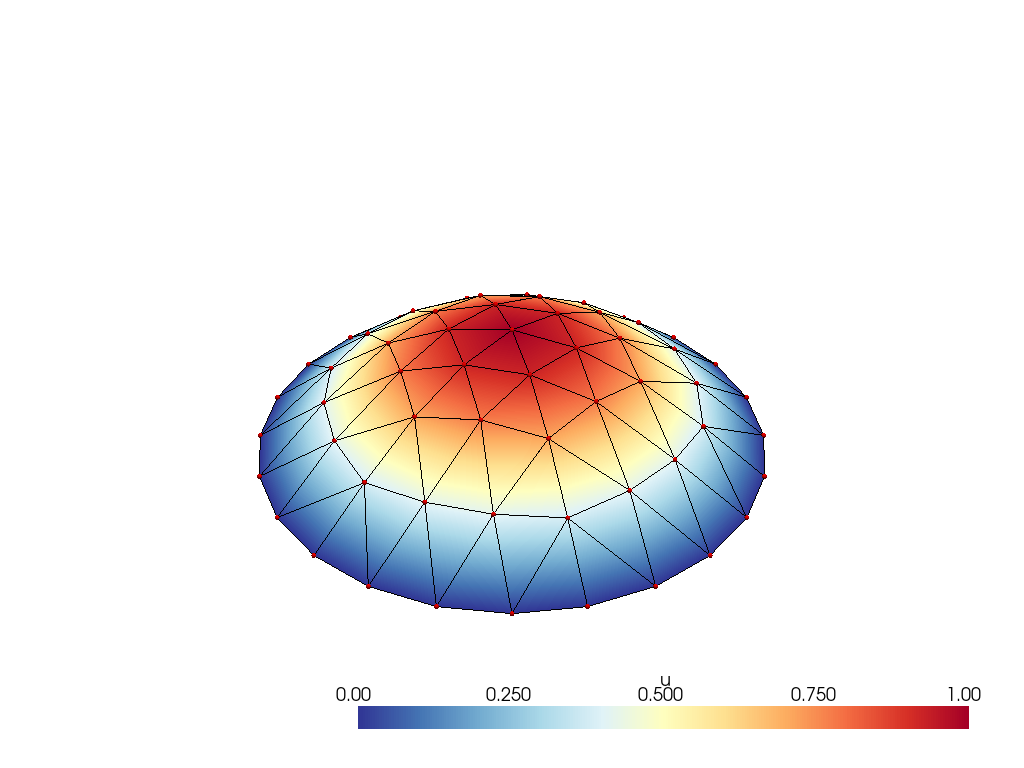
\includegraphics[width=0.5\textwidth,height=\textheight]{../img/mesh1-gauss08-b.png}
\caption{Finite element solution for problem 1 over mesh number 1 and
order-8 numerical integration.}
\end{figure}

\begin{figure}
\centering
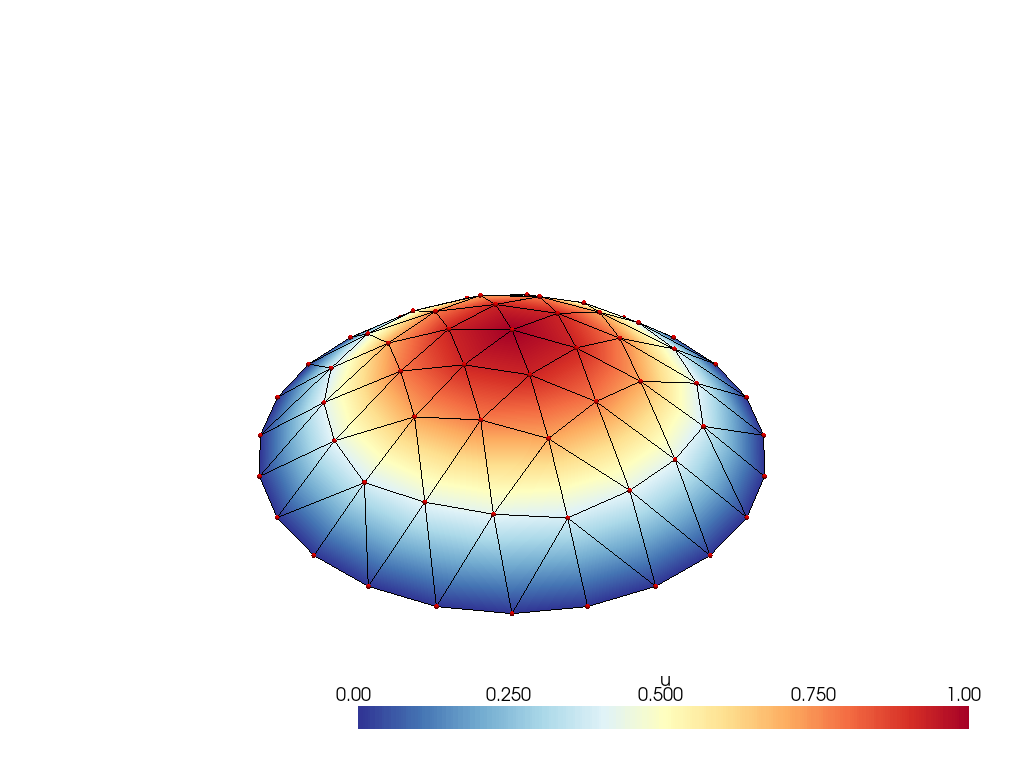
\includegraphics[width=0.5\textwidth,height=\textheight]{../img/mesh1-gauss13-b.png}
\caption{Finite element solution for problem 1 over mesh number 1 and
order-13 numerical integration.}
\end{figure}

\begin{figure}
\centering
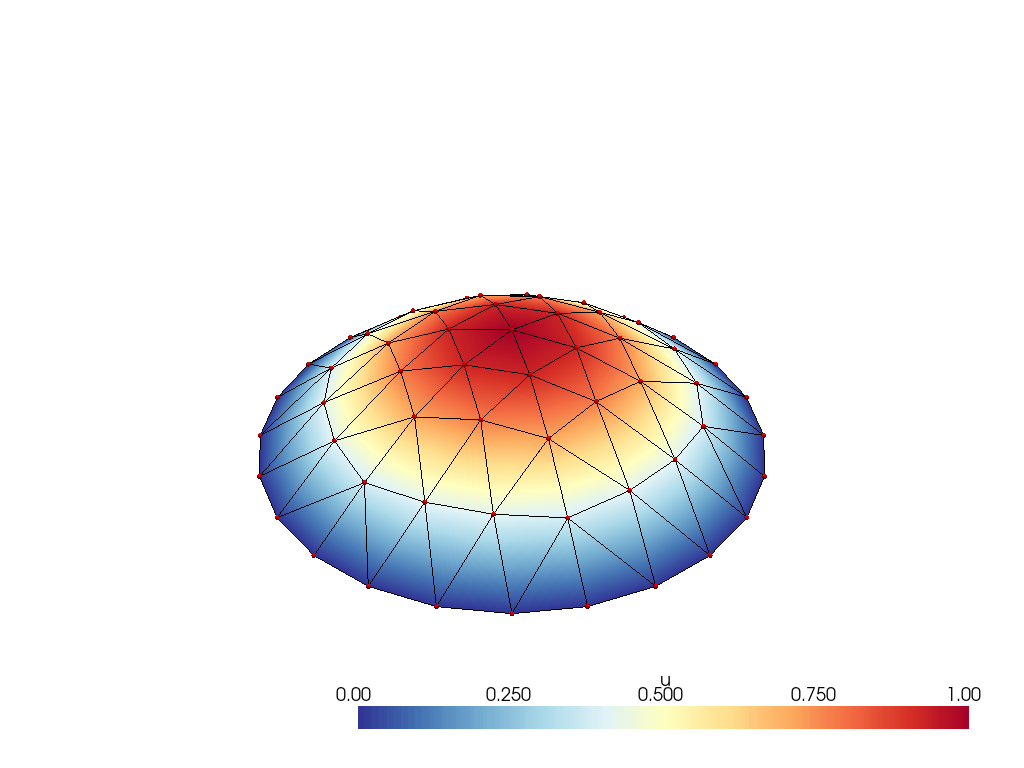
\includegraphics[width=0.5\textwidth,height=\textheight]{../img/mesh1-gauss19-b.png}
\caption{Finite element solution for problem 1 over mesh number 1 and
order-19 numerical integration.}
\end{figure}

\begin{figure}
\centering
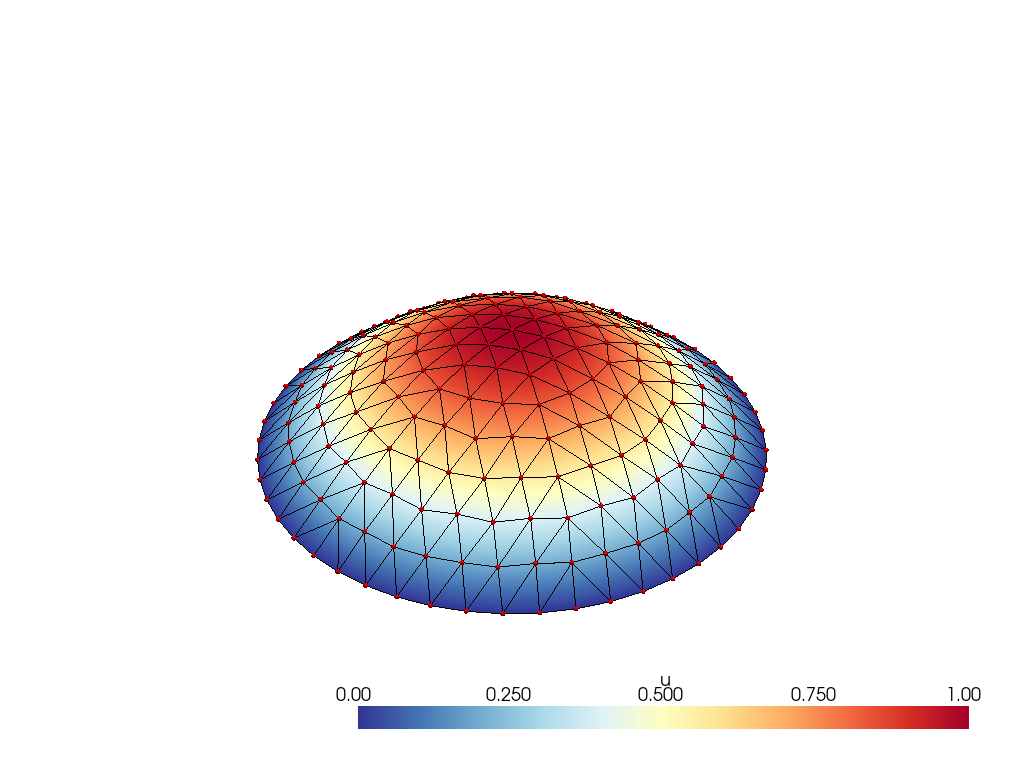
\includegraphics[width=0.5\textwidth,height=\textheight]{../img/mesh2-gauss02-b.png}
\caption{Finite element solution for problem 1 over mesh number 2 and
order-2 numerical integration.}
\end{figure}

\begin{figure}
\centering
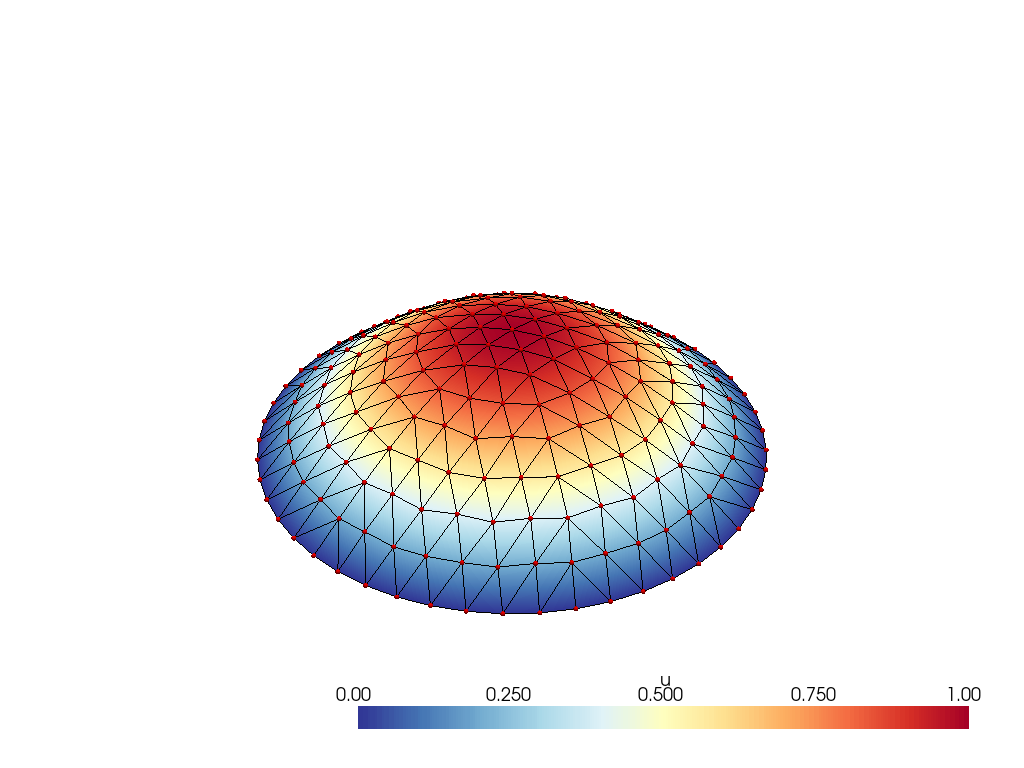
\includegraphics[width=0.5\textwidth,height=\textheight]{../img/mesh2-gauss05-b.png}
\caption{Finite element solution for problem 1 over mesh number 2 and
order-5 numerical integration.}
\end{figure}

\begin{figure}
\centering
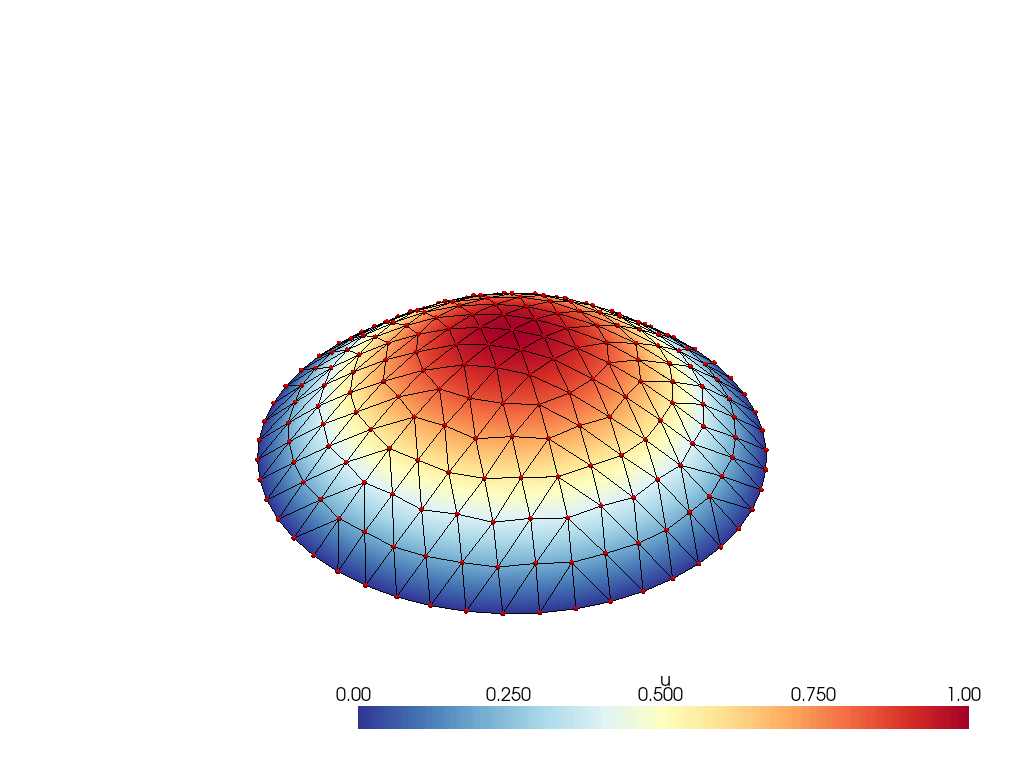
\includegraphics[width=0.5\textwidth,height=\textheight]{../img/mesh2-gauss08-b.png}
\caption{Finite element solution for problem 1 over mesh number 2 and
order-8 numerical integration.}
\end{figure}

\begin{figure}
\centering
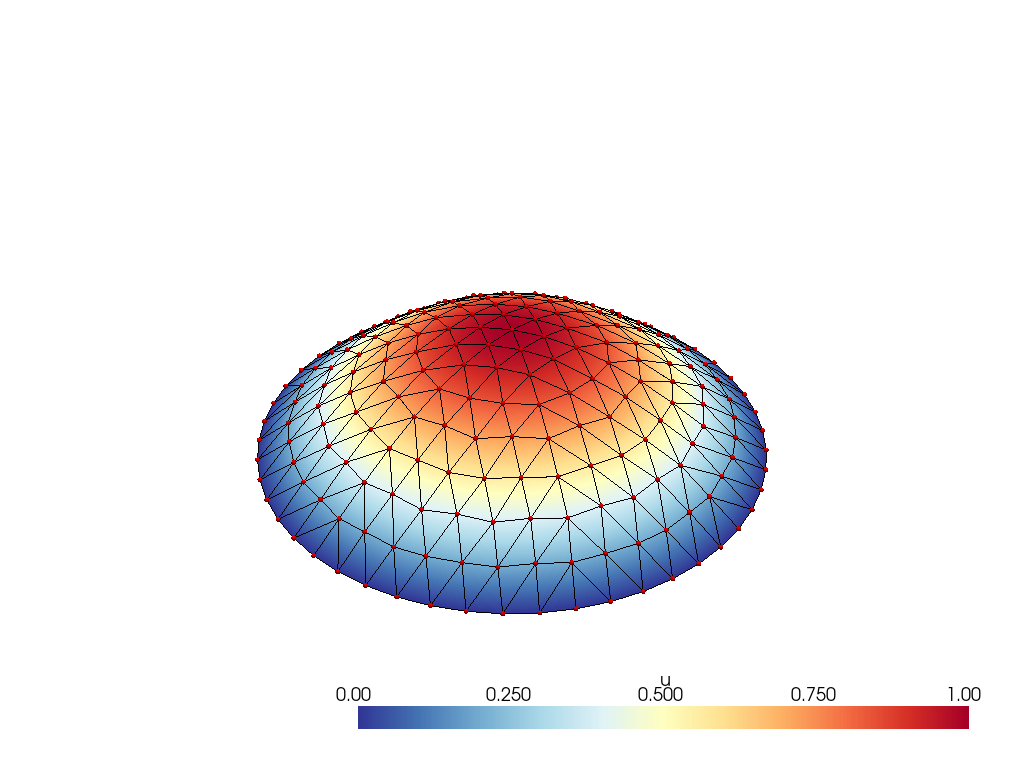
\includegraphics[width=0.5\textwidth,height=\textheight]{../img/mesh2-gauss13-b.png}
\caption{Finite element solution for problem 1 over mesh number 2 and
order-13 numerical integration.}
\end{figure}

\begin{figure}
\centering
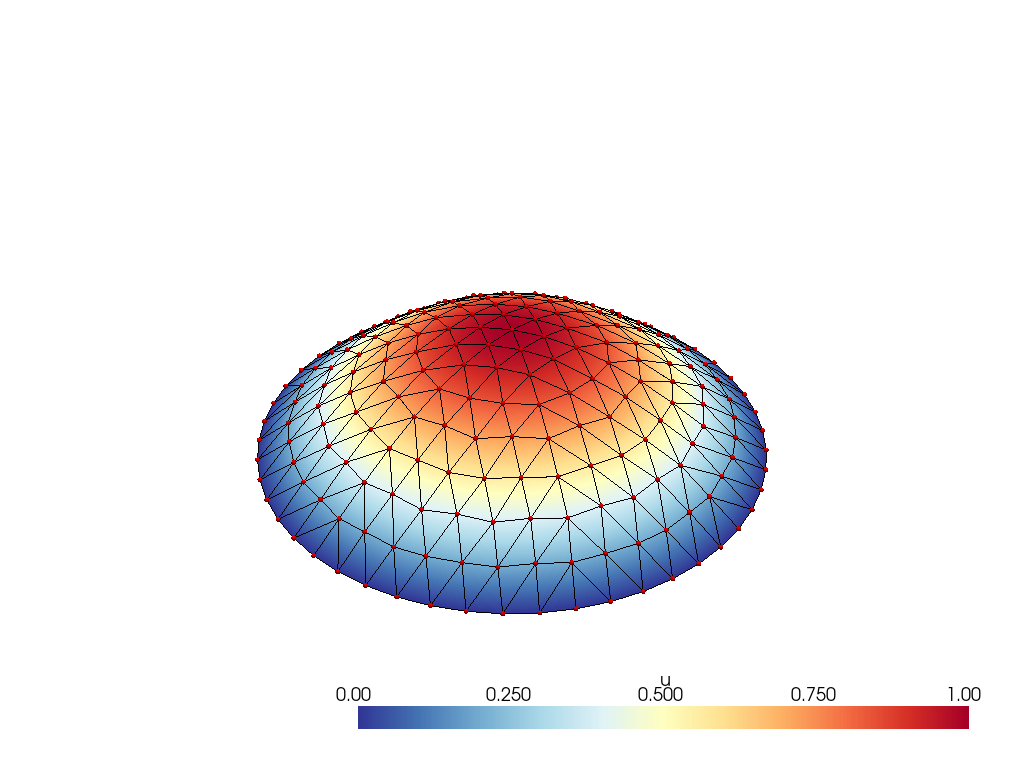
\includegraphics[width=0.5\textwidth,height=\textheight]{../img/mesh2-gauss19-b.png}
\caption{Finite element solution for problem 1 over mesh number 2 and
order-19 numerical integration.}
\end{figure}

\begin{figure}
\centering
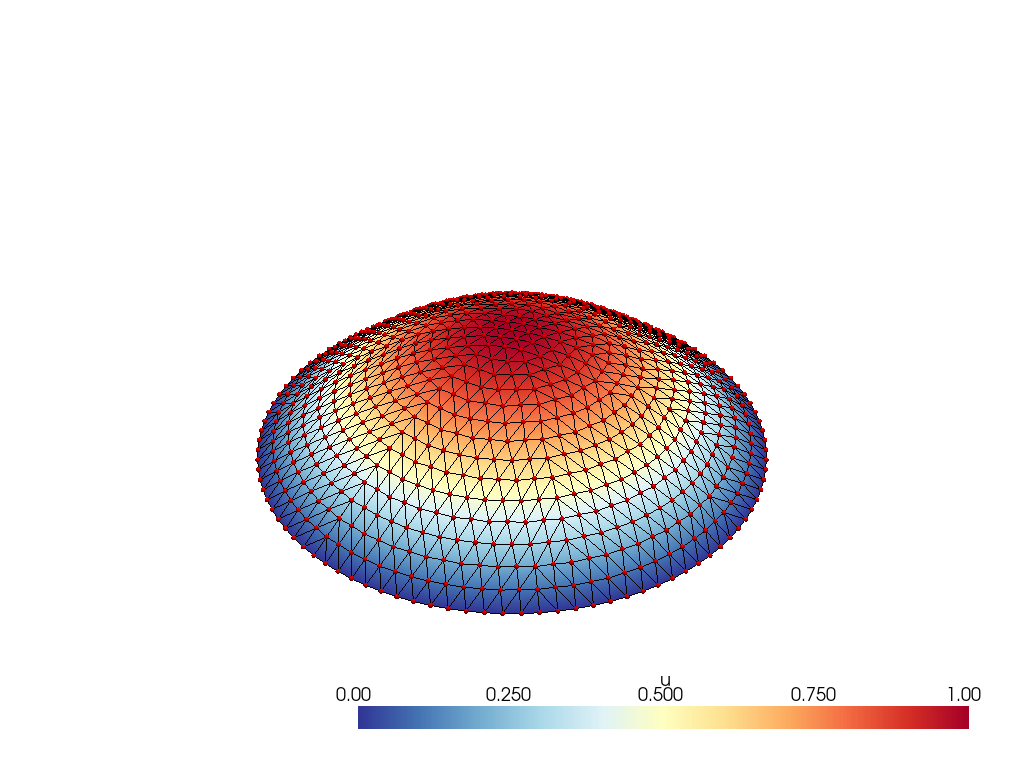
\includegraphics[width=0.5\textwidth,height=\textheight]{../img/mesh3-gauss02-b.png}
\caption{Finite element solution for problem 1 over mesh number 3 and
order-2 numerical integration.}
\end{figure}

\begin{figure}
\centering
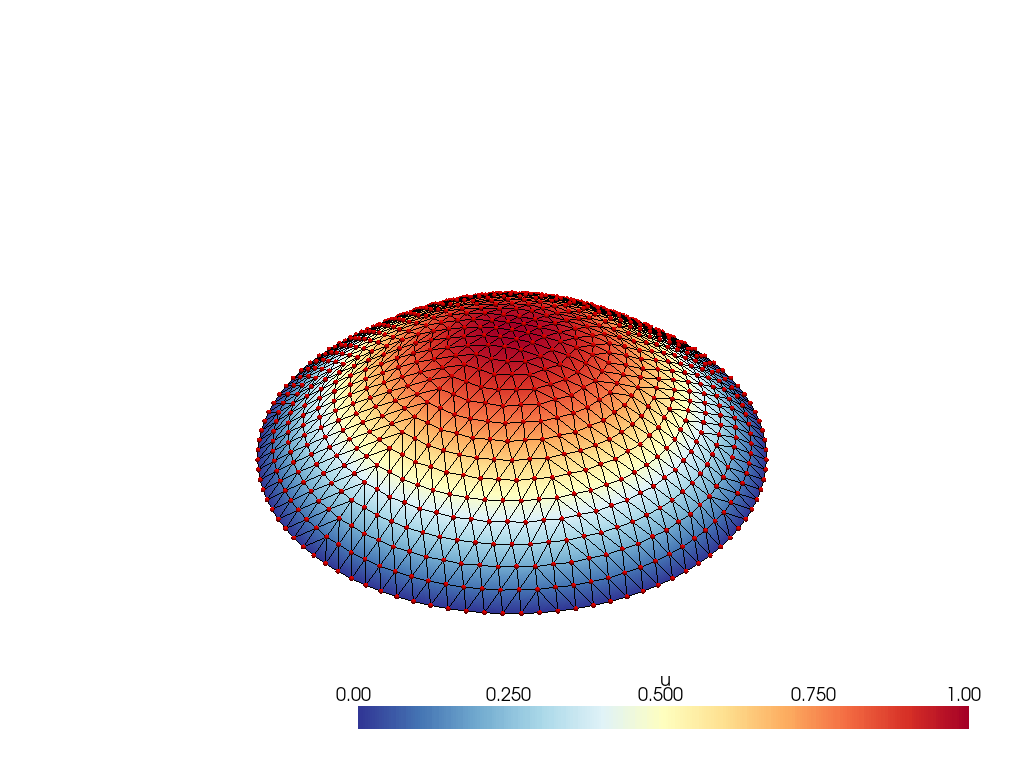
\includegraphics[width=0.5\textwidth,height=\textheight]{../img/mesh3-gauss05-b.png}
\caption{Finite element solution for problem 1 over mesh number 3 and
order-5 numerical integration.}
\end{figure}

\begin{figure}
\centering
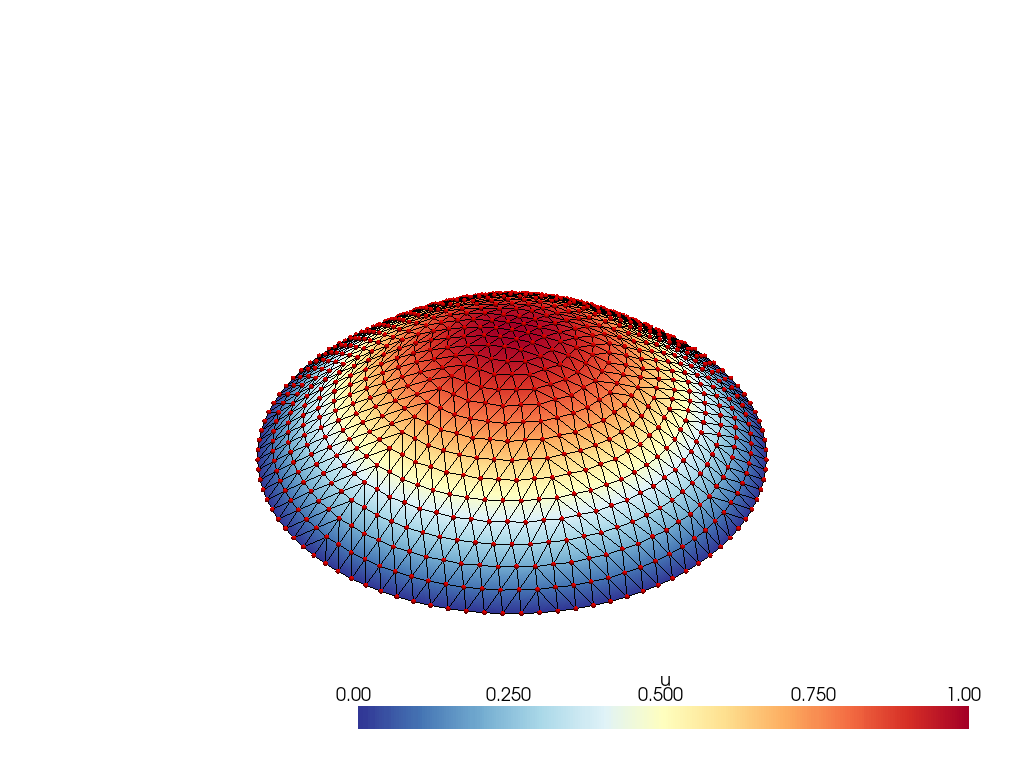
\includegraphics[width=0.5\textwidth,height=\textheight]{../img/mesh3-gauss08-b.png}
\caption{Finite element solution for problem 1 over mesh number 3 and
order-8 numerical integration.}
\end{figure}

\begin{figure}
\centering
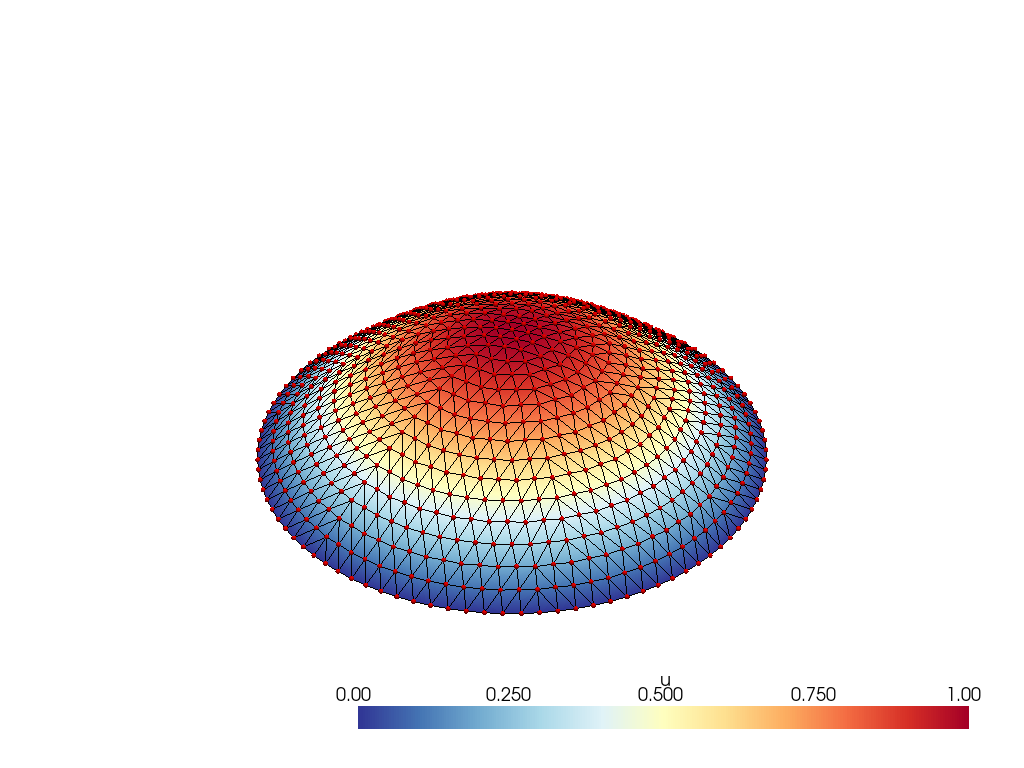
\includegraphics[width=0.5\textwidth,height=\textheight]{../img/mesh3-gauss13-b.png}
\caption{Finite element solution for problem 1 over mesh number 3 and
order-13 numerical integration.}
\end{figure}

\begin{figure}
\centering
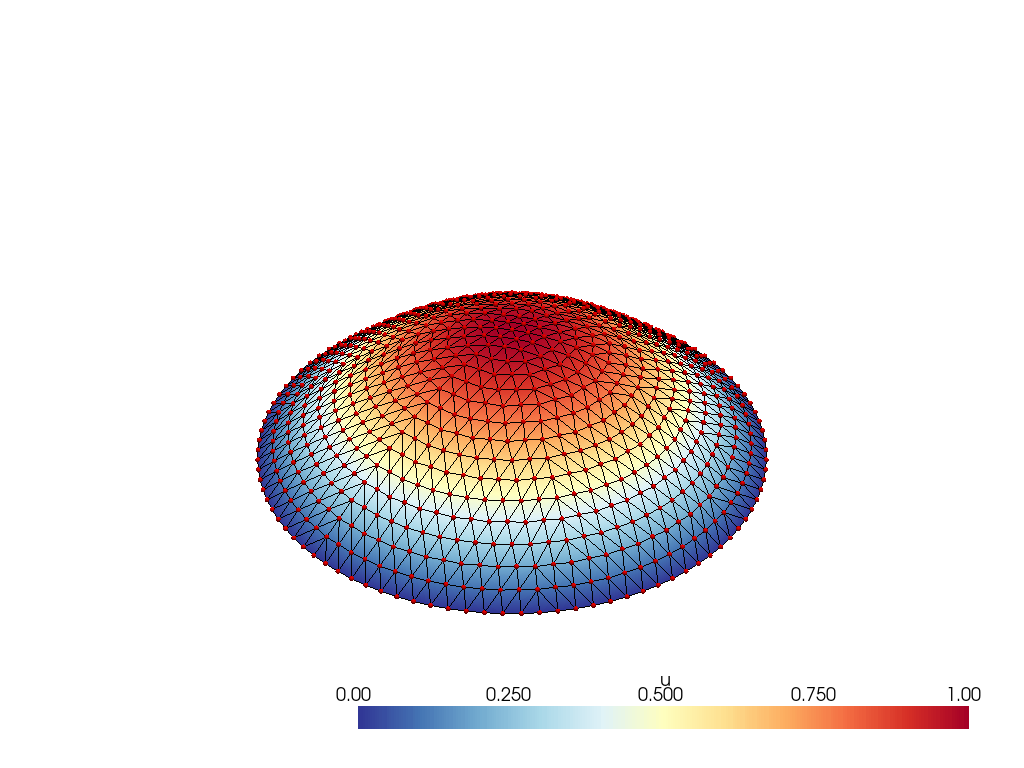
\includegraphics[width=0.5\textwidth,height=\textheight]{../img/mesh3-gauss19-b.png}
\caption{Finite element solution for problem 1 over mesh number 3 and
order-19 numerical integration.}
\end{figure}

\begin{figure}
\centering
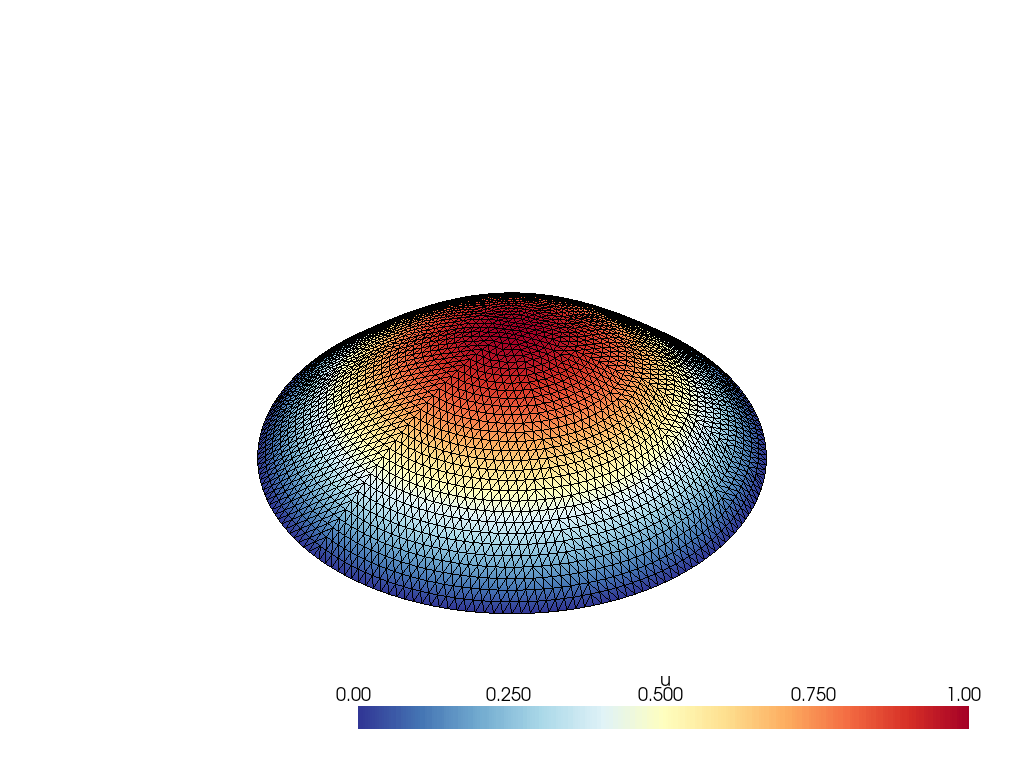
\includegraphics[width=0.5\textwidth,height=\textheight]{../img/mesh4-gauss02-b.png}
\caption{Finite element solution for problem 1 over mesh number 4 and
order-2 numerical integration.}
\end{figure}

\begin{figure}
\centering
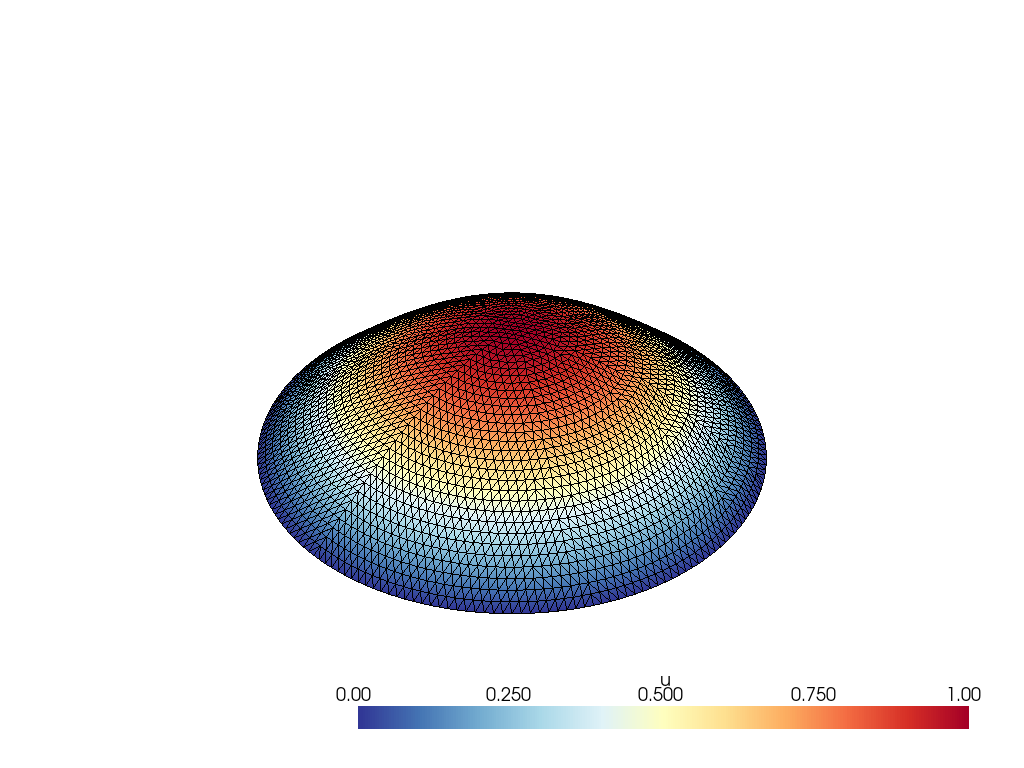
\includegraphics[width=0.5\textwidth,height=\textheight]{../img/mesh4-gauss05-b.png}
\caption{Finite element solution for problem 1 over mesh number 4 and
order-5 numerical integration.}
\end{figure}

\begin{figure}
\centering
\includegraphics[width=0.5\textwidth,height=\textheight]{../img/mesh4-gauss08-b.png}
\caption{Finite element solution for problem 1 over mesh number 4 and
order-8 numerical integration.}
\end{figure}

\begin{figure}
\centering
\includegraphics[width=0.5\textwidth,height=\textheight]{../img/mesh4-gauss13-b.png}
\caption{Finite element solution for problem 1 over mesh number 4 and
order-13 numerical integration.}
\end{figure}

\begin{figure}
\centering
\includegraphics[width=0.5\textwidth,height=\textheight]{../img/mesh4-gauss19-b.png}
\caption{Finite element solution for problem 1 over mesh number 4 and
order-19 numerical integration.}
\end{figure}

\begin{figure}
\centering
\includegraphics[width=0.5\textwidth,height=\textheight]{../img/mesh5-gauss02-b.png}
\caption{Finite element solution for problem 1 over mesh number 5 and
order-2 numerical integration.}
\end{figure}

\begin{figure}
\centering
\includegraphics[width=0.5\textwidth,height=\textheight]{../img/mesh5-gauss05-b.png}
\caption{Finite element solution for problem 1 over mesh number 5 and
order-5 numerical integration.}
\end{figure}

\begin{figure}
\centering
\includegraphics[width=0.5\textwidth,height=\textheight]{../img/mesh5-gauss08-b.png}
\caption{Finite element solution for problem 1 over mesh number 5 and
order-8 numerical integration.}
\end{figure}

\begin{figure}
\centering
\includegraphics[width=0.5\textwidth,height=\textheight]{../img/mesh5-gauss13-b.png}
\caption{Finite element solution for problem 1 over mesh number 5 and
order-13 numerical integration.}
\end{figure}

\begin{figure}
\centering
\includegraphics[width=0.5\textwidth,height=\textheight]{../img/mesh5-gauss19-b.png}
\caption{Finite element solution for problem 1 over mesh number 5 and
order-19 numerical integration.}
\end{figure}

\hypertarget{errors-in-the-h1-and-l2-norms}{%
\subsubsection{\texorpdfstring{Errors in the \(H^1\) and \(L2\)
norms}{Errors in the H\^{}1 and L2 norms}}\label{errors-in-the-h1-and-l2-norms}}

\includegraphics[width=0.5\textwidth,height=\textheight]{../img/mesh1-gauss02-L2.png}
\includegraphics[width=0.5\textwidth,height=\textheight]{../img/mesh1-gauss02-H1.png}

\begin{figure}
\caption{Finite element error in the L2 and H1 norms/seminorms, respectively for problem 1 over mesh number 1 using order 2 quadrature.}
\end{figure}

\includegraphics[width=0.5\textwidth,height=\textheight]{../img/mesh1-gauss05-L2.png}
\includegraphics[width=0.5\textwidth,height=\textheight]{../img/mesh1-gauss05-H1.png}

\begin{figure}
\caption{Finite element error in the L2 and H1 norms/seminorms, respectively for problem 1 over mesh number 1 using order 5 quadrature.}
\end{figure}

\includegraphics[width=0.5\textwidth,height=\textheight]{../img/mesh1-gauss08-L2.png}
\includegraphics[width=0.5\textwidth,height=\textheight]{../img/mesh1-gauss08-H1.png}

\begin{figure}
\caption{Finite element error in the L2 and H1 norms/seminorms, respectively for problem 1 over mesh number 1 using order 8 quadrature.}
\end{figure}

\includegraphics[width=0.5\textwidth,height=\textheight]{../img/mesh1-gauss13-L2.png}
\includegraphics[width=0.5\textwidth,height=\textheight]{../img/mesh1-gauss13-H1.png}

\begin{figure}
\caption{Finite element error in the L2 and H1 norms/seminorms, respectively for problem 1 over mesh number 1 using order 13 quadrature.}
\end{figure}

\includegraphics[width=0.5\textwidth,height=\textheight]{../img/mesh1-gauss19-L2.png}
\includegraphics[width=0.5\textwidth,height=\textheight]{../img/mesh1-gauss19-H1.png}

\begin{figure}
\caption{Finite element error in the L2 and H1 norms/seminorms, respectively for problem 1 over mesh number 1 using order 19 quadrature.}
\end{figure}

\includegraphics[width=0.5\textwidth,height=\textheight]{../img/mesh2-gauss02-L2.png}
\includegraphics[width=0.5\textwidth,height=\textheight]{../img/mesh2-gauss02-H1.png}

\begin{figure}
\caption{Finite element error in the L2 and H1 norms/seminorms, respectively for problem 1 over mesh number 2 using order 2 quadrature.}
\end{figure}

\includegraphics[width=0.5\textwidth,height=\textheight]{../img/mesh2-gauss05-L2.png}
\includegraphics[width=0.5\textwidth,height=\textheight]{../img/mesh2-gauss05-H1.png}

\begin{figure}
\caption{Finite element error in the L2 and H1 norms/seminorms, respectively for problem 1 over mesh number 2 using order 5 quadrature.}
\end{figure}

\includegraphics[width=0.5\textwidth,height=\textheight]{../img/mesh2-gauss08-L2.png}
\includegraphics[width=0.5\textwidth,height=\textheight]{../img/mesh2-gauss08-H1.png}

\begin{figure}
\caption{Finite element error in the L2 and H1 norms/seminorms, respectively for problem 1 over mesh number 2 using order 8 quadrature.}
\end{figure}

\includegraphics[width=0.5\textwidth,height=\textheight]{../img/mesh2-gauss13-L2.png}
\includegraphics[width=0.5\textwidth,height=\textheight]{../img/mesh2-gauss13-H1.png}

\begin{figure}
\caption{Finite element error in the L2 and H1 norms/seminorms, respectively for problem 1 over mesh number 2 using order 13 quadrature.}
\end{figure}

\includegraphics[width=0.5\textwidth,height=\textheight]{../img/mesh2-gauss19-L2.png}
\includegraphics[width=0.5\textwidth,height=\textheight]{../img/mesh2-gauss19-H1.png}

\begin{figure}
\caption{Finite element error in the L2 and H1 norms/seminorms, respectively for problem 1 over mesh number 2 using order 19 quadrature.}
\end{figure}

\includegraphics[width=0.5\textwidth,height=\textheight]{../img/mesh3-gauss02-L2.png}
\includegraphics[width=0.5\textwidth,height=\textheight]{../img/mesh3-gauss02-H1.png}

\begin{figure}
\caption{Finite element error in the L2 and H1 norms/seminorms, respectively for problem 1 over mesh number 3 using order 2 quadrature.}
\end{figure}

\includegraphics[width=0.5\textwidth,height=\textheight]{../img/mesh3-gauss05-L2.png}
\includegraphics[width=0.5\textwidth,height=\textheight]{../img/mesh3-gauss05-H1.png}

\begin{figure}
\caption{Finite element error in the L2 and H1 norms/seminorms, respectively for problem 1 over mesh number 3 using order 5 quadrature.}
\end{figure}

\includegraphics[width=0.5\textwidth,height=\textheight]{../img/mesh3-gauss08-L2.png}
\includegraphics[width=0.5\textwidth,height=\textheight]{../img/mesh3-gauss08-H1.png}

\begin{figure}
\caption{Finite element error in the L2 and H1 norms/seminorms, respectively for problem 1 over mesh number 3 using order 8 quadrature.}
\end{figure}

\includegraphics[width=0.5\textwidth,height=\textheight]{../img/mesh3-gauss13-L2.png}
\includegraphics[width=0.5\textwidth,height=\textheight]{../img/mesh3-gauss13-H1.png}

\begin{figure}
\caption{Finite element error in the L2 and H1 norms/seminorms, respectively for problem 1 over mesh number 3 using order 13 quadrature.}
\end{figure}

\includegraphics[width=0.5\textwidth,height=\textheight]{../img/mesh3-gauss19-L2.png}
\includegraphics[width=0.5\textwidth,height=\textheight]{../img/mesh3-gauss19-H1.png}

\begin{figure}
\caption{Finite element error in the L2 and H1 norms/seminorms, respectively for problem 1 over mesh number 3 using order 19 quadrature.}
\end{figure}

\includegraphics[width=0.5\textwidth,height=\textheight]{../img/mesh4-gauss02-L2.png}
\includegraphics[width=0.5\textwidth,height=\textheight]{../img/mesh4-gauss02-H1.png}

\begin{figure}
\caption{Finite element error in the L2 and H1 norms/seminorms, respectively for problem 1 over mesh number 4 using order 2 quadrature.}
\end{figure}

\includegraphics[width=0.5\textwidth,height=\textheight]{../img/mesh4-gauss05-L2.png}
\includegraphics[width=0.5\textwidth,height=\textheight]{../img/mesh4-gauss05-H1.png}

\begin{figure}
\caption{Finite element error in the L2 and H1 norms/seminorms, respectively for problem 1 over mesh number 4 using order 5 quadrature.}
\end{figure}

\includegraphics[width=0.5\textwidth,height=\textheight]{../img/mesh4-gauss08-L2.png}
\includegraphics[width=0.5\textwidth,height=\textheight]{../img/mesh4-gauss08-H1.png}

\begin{figure}
\caption{Finite element error in the L2 and H1 norms/seminorms, respectively for problem 1 over mesh number 4 using order 8 quadrature.}
\end{figure}

\includegraphics[width=0.5\textwidth,height=\textheight]{../img/mesh4-gauss13-L2.png}
\includegraphics[width=0.5\textwidth,height=\textheight]{../img/mesh4-gauss13-H1.png}

\begin{figure}
\caption{Finite element error in the L2 and H1 norms/seminorms, respectively for problem 1 over mesh number 4 using order 13 quadrature.}
\end{figure}

\includegraphics[width=0.5\textwidth,height=\textheight]{../img/mesh4-gauss19-L2.png}
\includegraphics[width=0.5\textwidth,height=\textheight]{../img/mesh4-gauss19-H1.png}

\begin{figure}
\caption{Finite element error in the L2 and H1 norms/seminorms, respectively for problem 1 over mesh number 4 using order 19 quadrature.}
\end{figure}

\includegraphics[width=0.5\textwidth,height=\textheight]{../img/mesh5-gauss02-L2.png}
\includegraphics[width=0.5\textwidth,height=\textheight]{../img/mesh5-gauss02-H1.png}

\begin{figure}
\caption{Finite element error in the L2 and H1 norms/seminorms, respectively for problem 1 over mesh number 5 using order 2 quadrature.}
\end{figure}

\includegraphics[width=0.5\textwidth,height=\textheight]{../img/mesh5-gauss05-L2.png}
\includegraphics[width=0.5\textwidth,height=\textheight]{../img/mesh5-gauss05-H1.png}

\begin{figure}
\caption{Finite element error in the L2 and H1 norms/seminorms, respectively for problem 1 over mesh number 5 using order 5 quadrature.}
\end{figure}

\includegraphics[width=0.5\textwidth,height=\textheight]{../img/mesh5-gauss08-L2.png}
\includegraphics[width=0.5\textwidth,height=\textheight]{../img/mesh5-gauss08-H1.png}

\begin{figure}
\caption{Finite element error in the L2 and H1 norms/seminorms, respectively for problem 1 over mesh number 5 using order 8 quadrature.}
\end{figure}

\includegraphics[width=0.5\textwidth,height=\textheight]{../img/mesh5-gauss13-L2.png}
\includegraphics[width=0.5\textwidth,height=\textheight]{../img/mesh5-gauss13-H1.png}

\begin{figure}
\caption{Finite element error in the L2 and H1 norms/seminorms, respectively for problem 1 over mesh number 5 using order 13 quadrature.}
\end{figure}

\includegraphics[width=0.5\textwidth,height=\textheight]{../img/mesh5-gauss19-L2.png}
\includegraphics[width=0.5\textwidth,height=\textheight]{../img/mesh5-gauss19-H1.png}

\begin{figure}
\caption{Finite element error in the L2 and H1 norms/seminorms, respectively for problem 1 over mesh number 5 using order 19 quadrature.}
\end{figure}

\includegraphics[width=0.5\textwidth,height=\textheight]{../img/mesh1-gauss02-b-L2.png}
\includegraphics[width=0.5\textwidth,height=\textheight]{../img/mesh1-gauss02-b-H1.png}

\begin{figure}
\caption{Finite element error in the L2 and H1 norms/seminorms, respectively for problem 1 over mesh number 1 using order 2 quadrature.}
\end{figure}

\includegraphics[width=0.5\textwidth,height=\textheight]{../img/mesh1-gauss05-b-L2.png}
\includegraphics[width=0.5\textwidth,height=\textheight]{../img/mesh1-gauss05-b-H1.png}

\begin{figure}
\caption{Finite element error in the L2 and H1 norms/seminorms, respectively for problem 1 over mesh number 1 using order 5 quadrature.}
\end{figure}

\includegraphics[width=0.5\textwidth,height=\textheight]{../img/mesh1-gauss08-b-L2.png}
\includegraphics[width=0.5\textwidth,height=\textheight]{../img/mesh1-gauss08-b-H1.png}

\begin{figure}
\caption{Finite element error in the L2 and H1 norms/seminorms, respectively for problem 1 over mesh number 1 using order 8 quadrature.}
\end{figure}

\includegraphics[width=0.5\textwidth,height=\textheight]{../img/mesh1-gauss13-b-L2.png}
\includegraphics[width=0.5\textwidth,height=\textheight]{../img/mesh1-gauss13-b-H1.png}

\begin{figure}
\caption{Finite element error in the L2 and H1 norms/seminorms, respectively for problem 1 over mesh number 1 using order 13 quadrature.}
\end{figure}

\includegraphics[width=0.5\textwidth,height=\textheight]{../img/mesh1-gauss19-b-L2.png}
\includegraphics[width=0.5\textwidth,height=\textheight]{../img/mesh1-gauss19-b-H1.png}

\begin{figure}
\caption{Finite element error in the L2 and H1 norms/seminorms, respectively for problem 1 over mesh number 1 using order 19 quadrature.}
\end{figure}

\includegraphics[width=0.5\textwidth,height=\textheight]{../img/mesh2-gauss02-b-L2.png}
\includegraphics[width=0.5\textwidth,height=\textheight]{../img/mesh2-gauss02-b-H1.png}

\begin{figure}
\caption{Finite element error in the L2 and H1 norms/seminorms, respectively for problem 1 over mesh number 2 using order 2 quadrature.}
\end{figure}

\includegraphics[width=0.5\textwidth,height=\textheight]{../img/mesh2-gauss05-b-L2.png}
\includegraphics[width=0.5\textwidth,height=\textheight]{../img/mesh2-gauss05-b-H1.png}

\begin{figure}
\caption{Finite element error in the L2 and H1 norms/seminorms, respectively for problem 1 over mesh number 2 using order 5 quadrature.}
\end{figure}

\includegraphics[width=0.5\textwidth,height=\textheight]{../img/mesh2-gauss08-b-L2.png}
\includegraphics[width=0.5\textwidth,height=\textheight]{../img/mesh2-gauss08-b-H1.png}

\begin{figure}
\caption{Finite element error in the L2 and H1 norms/seminorms, respectively for problem 1 over mesh number 2 using order 8 quadrature.}
\end{figure}

\includegraphics[width=0.5\textwidth,height=\textheight]{../img/mesh2-gauss13-b-L2.png}
\includegraphics[width=0.5\textwidth,height=\textheight]{../img/mesh2-gauss13-b-H1.png}

\begin{figure}
\caption{Finite element error in the L2 and H1 norms/seminorms, respectively for problem 1 over mesh number 2 using order 13 quadrature.}
\end{figure}

\includegraphics[width=0.5\textwidth,height=\textheight]{../img/mesh2-gauss19-b-L2.png}
\includegraphics[width=0.5\textwidth,height=\textheight]{../img/mesh2-gauss19-b-H1.png}

\begin{figure}
\caption{Finite element error in the L2 and H1 norms/seminorms, respectively for problem 1 over mesh number 2 using order 19 quadrature.}
\end{figure}

\includegraphics[width=0.5\textwidth,height=\textheight]{../img/mesh3-gauss02-b-L2.png}
\includegraphics[width=0.5\textwidth,height=\textheight]{../img/mesh3-gauss02-b-H1.png}

\begin{figure}
\caption{Finite element error in the L2 and H1 norms/seminorms, respectively for problem 1 over mesh number 3 using order 2 quadrature.}
\end{figure}

\includegraphics[width=0.5\textwidth,height=\textheight]{../img/mesh3-gauss05-b-L2.png}
\includegraphics[width=0.5\textwidth,height=\textheight]{../img/mesh3-gauss05-b-H1.png}

\begin{figure}
\caption{Finite element error in the L2 and H1 norms/seminorms, respectively for problem 1 over mesh number 3 using order 5 quadrature.}
\end{figure}

\includegraphics[width=0.5\textwidth,height=\textheight]{../img/mesh3-gauss08-b-L2.png}
\includegraphics[width=0.5\textwidth,height=\textheight]{../img/mesh3-gauss08-b-H1.png}

\begin{figure}
\caption{Finite element error in the L2 and H1 norms/seminorms, respectively for problem 1 over mesh number 3 using order 8 quadrature.}
\end{figure}

\includegraphics[width=0.5\textwidth,height=\textheight]{../img/mesh3-gauss13-b-L2.png}
\includegraphics[width=0.5\textwidth,height=\textheight]{../img/mesh3-gauss13-b-H1.png}

\begin{figure}
\caption{Finite element error in the L2 and H1 norms/seminorms, respectively for problem 1 over mesh number 3 using order 13 quadrature.}
\end{figure}

\includegraphics[width=0.5\textwidth,height=\textheight]{../img/mesh3-gauss19-b-L2.png}
\includegraphics[width=0.5\textwidth,height=\textheight]{../img/mesh3-gauss19-b-H1.png}

\begin{figure}
\caption{Finite element error in the L2 and H1 norms/seminorms, respectively for problem 1 over mesh number 3 using order 19 quadrature.}
\end{figure}

\includegraphics[width=0.5\textwidth,height=\textheight]{../img/mesh4-gauss02-b-L2.png}
\includegraphics[width=0.5\textwidth,height=\textheight]{../img/mesh4-gauss02-b-H1.png}

\begin{figure}
\caption{Finite element error in the L2 and H1 norms/seminorms, respectively for problem 1 over mesh number 4 using order 2 quadrature.}
\end{figure}

\includegraphics[width=0.5\textwidth,height=\textheight]{../img/mesh4-gauss05-b-L2.png}
\includegraphics[width=0.5\textwidth,height=\textheight]{../img/mesh4-gauss05-b-H1.png}

\begin{figure}
\caption{Finite element error in the L2 and H1 norms/seminorms, respectively for problem 1 over mesh number 4 using order 5 quadrature.}
\end{figure}

\includegraphics[width=0.5\textwidth,height=\textheight]{../img/mesh4-gauss08-b-L2.png}
\includegraphics[width=0.5\textwidth,height=\textheight]{../img/mesh4-gauss08-b-H1.png}

\begin{figure}
\caption{Finite element error in the L2 and H1 norms/seminorms, respectively for problem 1 over mesh number 4 using order 8 quadrature.}
\end{figure}

\includegraphics[width=0.5\textwidth,height=\textheight]{../img/mesh4-gauss13-b-L2.png}
\includegraphics[width=0.5\textwidth,height=\textheight]{../img/mesh4-gauss13-b-H1.png}

\begin{figure}
\caption{Finite element error in the L2 and H1 norms/seminorms, respectively for problem 1 over mesh number 4 using order 13 quadrature.}
\end{figure}

\includegraphics[width=0.5\textwidth,height=\textheight]{../img/mesh4-gauss19-b-L2.png}
\includegraphics[width=0.5\textwidth,height=\textheight]{../img/mesh4-gauss19-b-H1.png}

\begin{figure}
\caption{Finite element error in the L2 and H1 norms/seminorms, respectively for problem 1 over mesh number 4 using order 19 quadrature.}
\end{figure}

\includegraphics[width=0.5\textwidth,height=\textheight]{../img/mesh5-gauss02-b-L2.png}
\includegraphics[width=0.5\textwidth,height=\textheight]{../img/mesh5-gauss02-b-H1.png}

\begin{figure}
\caption{Finite element error in the L2 and H1 norms/seminorms, respectively for problem 1 over mesh number 5 using order 2 quadrature.}
\end{figure}

\includegraphics[width=0.5\textwidth,height=\textheight]{../img/mesh5-gauss05-b-L2.png}
\includegraphics[width=0.5\textwidth,height=\textheight]{../img/mesh5-gauss05-b-H1.png}

\begin{figure}
\caption{Finite element error in the L2 and H1 norms/seminorms, respectively for problem 1 over mesh number 5 using order 5 quadrature.}
\end{figure}

\includegraphics[width=0.5\textwidth,height=\textheight]{../img/mesh5-gauss08-b-L2.png}
\includegraphics[width=0.5\textwidth,height=\textheight]{../img/mesh5-gauss08-b-H1.png}

\begin{figure}
\caption{Finite element error in the L2 and H1 norms/seminorms, respectively for problem 1 over mesh number 5 using order 8 quadrature.}
\end{figure}

\includegraphics[width=0.5\textwidth,height=\textheight]{../img/mesh5-gauss13-b-L2.png}
\includegraphics[width=0.5\textwidth,height=\textheight]{../img/mesh5-gauss13-b-H1.png}

\begin{figure}
\caption{Finite element error in the L2 and H1 norms/seminorms, respectively for problem 1 over mesh number 5 using order 13 quadrature.}
\end{figure}

\includegraphics[width=0.5\textwidth,height=\textheight]{../img/mesh5-gauss19-b-L2.png}
\includegraphics[width=0.5\textwidth,height=\textheight]{../img/mesh5-gauss19-b-H1.png}

\begin{figure}
\caption{Finite element error in the L2 and H1 norms/seminorms, respectively for problem 1 over mesh number 5 using order 19 quadrature.}
\end{figure}

\newpage{}

\hypertarget{source-code-of-interest}{%
\subsection{Source Code of Interest}\label{source-code-of-interest}}

\begin{Shaded}
\begin{Highlighting}[]
\CommentTok{\# Claudio Perez}
\CommentTok{\# May 2021}
\ImportTok{import}\NormalTok{ jax}
\ImportTok{import}\NormalTok{ anon.diff }\ImportTok{as}\NormalTok{ diff}
\ImportTok{from}\NormalTok{ anabel.template }\ImportTok{import}\NormalTok{ template}
\ImportTok{import}\NormalTok{ anabel.backend }\ImportTok{as}\NormalTok{ anp}


\AttributeTok{@template}\NormalTok{(}\DecValTok{6}\NormalTok{)}
\KeywordTok{def}\NormalTok{ poisson2(transf, test, trial, f}\OperatorTok{=}\KeywordTok{lambda}\NormalTok{ x: }\FloatTok{0.0}\NormalTok{, ndim}\OperatorTok{=}\DecValTok{2}\NormalTok{, points}\OperatorTok{=}\VariableTok{None}\NormalTok{, weights}\OperatorTok{=}\VariableTok{None}\NormalTok{, thickness}\OperatorTok{=}\FloatTok{1.0}\NormalTok{, }\OperatorTok{**}\NormalTok{kwds):}
    \CommentTok{"""}
\CommentTok{    Parameters}
\CommentTok{    {-}{-}{-}{-}{-}{-}{-}{-}{-}{-}}
\CommentTok{    test, trial : Callable}
\CommentTok{        test and trial interpolants over the reference element.}
\CommentTok{    thickness : float}
\CommentTok{    }
\CommentTok{    http://people.inf.ethz.ch/arbenz/FEM17/pdfs/0{-}19{-}852868{-}X.pdf}
\CommentTok{    """}
\NormalTok{    state }\OperatorTok{=}\NormalTok{ \{\}}
    
\NormalTok{    det }\OperatorTok{=}\NormalTok{ anp.linalg.det}
\NormalTok{    slv }\OperatorTok{=}\NormalTok{ anp.linalg.solve}
    
\NormalTok{    jacn\_test }\OperatorTok{=}\NormalTok{ diff.jacx(test)}
\NormalTok{    jacn\_trial }\OperatorTok{=}\NormalTok{ diff.jacx(trial)}
    
    \KeywordTok{def}\NormalTok{ transf(xi, xyz):}
        \ControlFlowTok{return}\NormalTok{ test(xi)}\OperatorTok{@}\NormalTok{xyz}
    
    \KeywordTok{def}\NormalTok{ jacn\_transf(xi,xyz):}
        \ControlFlowTok{return}\NormalTok{ jacn\_test(xi)}\OperatorTok{@}\NormalTok{xyz}
    
    \KeywordTok{def}\NormalTok{ jacx\_test(xi,xyz): }
        \ControlFlowTok{return}\NormalTok{ slv(jacn\_transf(xi,xyz), jacn\_test(xi))}
    
    \KeywordTok{def}\NormalTok{ dvol(xi, xyz): }
        \ControlFlowTok{return} \FloatTok{0.5}\OperatorTok{*}\NormalTok{thickness}\OperatorTok{*}\NormalTok{(}\BuiltInTok{abs}\NormalTok{(det(jacn\_transf(xi,xyz))))}
    
    \KeywordTok{def}\NormalTok{ stif(u,xyz,xi,wght,}\OperatorTok{**}\NormalTok{kwds):}
\NormalTok{        dNdx }\OperatorTok{=}\NormalTok{ jacx\_test(xi,xyz)}
        \ControlFlowTok{return}\NormalTok{ (dNdx.T}\OperatorTok{@}\NormalTok{dNdx)}\OperatorTok{*}\NormalTok{dvol(xi,xyz)}\OperatorTok{*}\NormalTok{wght}
    
\NormalTok{    fj }\OperatorTok{=}\NormalTok{ jax.vmap(f,}\DecValTok{0}\NormalTok{)}
    
    \KeywordTok{def}\NormalTok{ resp(u,xyz,xi,wght,}\OperatorTok{**}\NormalTok{kwds):}
\NormalTok{        dNdx }\OperatorTok{=}\NormalTok{ jacx\_test(xi,xyz)}
\NormalTok{        N }\OperatorTok{=}\NormalTok{ test(xi)[:,}\VariableTok{None}\NormalTok{]}
\NormalTok{        p }\OperatorTok{=}\NormalTok{ (dNdx.T}\OperatorTok{@}\NormalTok{dNdx)}\OperatorTok{@}\NormalTok{u}\OperatorTok{*}\NormalTok{dvol(xi,xyz)}\OperatorTok{*}\NormalTok{wght }\OperatorTok{{-}}\NormalTok{ (N}\OperatorTok{@}\NormalTok{N.T)}\OperatorTok{@}\NormalTok{fj(xyz)[:,}\VariableTok{None}\NormalTok{]}\OperatorTok{*}\NormalTok{dvol(xi,xyz)}\OperatorTok{*}\NormalTok{wght}
        \ControlFlowTok{return}\NormalTok{ p}
    
\NormalTok{    integral }\OperatorTok{=}\NormalTok{ jax.vmap(resp,(}\VariableTok{None}\NormalTok{,}\VariableTok{None}\NormalTok{,}\DecValTok{0}\NormalTok{,}\DecValTok{0}\NormalTok{))}
\NormalTok{    jac\_integral }\OperatorTok{=}\NormalTok{ jax.vmap(stif,(}\VariableTok{None}\NormalTok{, }\VariableTok{None}\NormalTok{, }\DecValTok{0}\NormalTok{, }\DecValTok{0}\NormalTok{))}
    
    \KeywordTok{def}\NormalTok{ jacx(u,\_\_,\_\_\_,xyz,points,weights):}
        \ControlFlowTok{return} \BuiltInTok{sum}\NormalTok{(jac\_integral(u,xyz,points,weights))}

    \KeywordTok{def}\NormalTok{ main(u,\_\_,\_\_\_,xyz,points,weights):}
        \ControlFlowTok{return} \BuiltInTok{sum}\NormalTok{(integral(u,xyz,points,weights))}
    \ControlFlowTok{return} \BuiltInTok{locals}\NormalTok{()}

\AttributeTok{@template}\NormalTok{(}\DecValTok{1}\NormalTok{)}
\KeywordTok{def}\NormalTok{ L2(transf,test,trial,u,quad\_point}\OperatorTok{=}\VariableTok{None}\NormalTok{, thickness}\OperatorTok{=}\FloatTok{1.0}\NormalTok{):}
\NormalTok{    state }\OperatorTok{=} \VariableTok{None}
\NormalTok{    det }\OperatorTok{=}\NormalTok{ anp.linalg.det}
\NormalTok{    slv }\OperatorTok{=}\NormalTok{ anp.linalg.solve}
\NormalTok{    du }\OperatorTok{=} \KeywordTok{lambda}\NormalTok{ x: diff.jacfwd(u)(x)[:,}\VariableTok{None}\NormalTok{]}
\NormalTok{    jacn\_test }\OperatorTok{=}\NormalTok{ diff.jacx(test)}
\NormalTok{    jacn\_trial }\OperatorTok{=}\NormalTok{ diff.jacx(trial)}

    \KeywordTok{def}\NormalTok{ transf(xi, xyz):}
        \ControlFlowTok{return}\NormalTok{ test(xi)}\OperatorTok{@}\NormalTok{xyz}
    
    \KeywordTok{def}\NormalTok{ jacn\_transf(xi,xyz):}
        \ControlFlowTok{return}\NormalTok{ jacn\_test(xi)}\OperatorTok{@}\NormalTok{xyz}

\NormalTok{    dvol }\OperatorTok{=} \KeywordTok{lambda}\NormalTok{ xi, xyz: }\FloatTok{0.5}\OperatorTok{*}\NormalTok{thickness}\OperatorTok{*}\BuiltInTok{abs}\NormalTok{(det(jacn\_transf(xi,xyz)))}
     
    \KeywordTok{def}\NormalTok{ resp(U,xyz,xi, wght):}
\NormalTok{        N }\OperatorTok{=}\NormalTok{ test(xi)[:,}\VariableTok{None}\NormalTok{]}
\NormalTok{        tmp }\OperatorTok{=}\NormalTok{ u(transf(xi,xyz)) }\OperatorTok{{-}}\NormalTok{ N.T}\OperatorTok{@}\NormalTok{U}
\NormalTok{        q }\OperatorTok{=}\NormalTok{  tmp.T}\OperatorTok{@}\NormalTok{tmp }\OperatorTok{*}\NormalTok{ dvol(xi,xyz) }\OperatorTok{*}\NormalTok{ wght}
        \ControlFlowTok{return}\NormalTok{ q}
    
\NormalTok{    integral }\OperatorTok{=}\NormalTok{ jax.vmap(resp,(}\VariableTok{None}\NormalTok{,}\VariableTok{None}\NormalTok{,}\DecValTok{0}\NormalTok{,}\DecValTok{0}\NormalTok{))}

    \KeywordTok{def}\NormalTok{ main(u,\_\_,\_\_\_,xyz,points,weights):}
        \ControlFlowTok{return} \BuiltInTok{sum}\NormalTok{(integral(u,xyz,points,weights))}
    
    \ControlFlowTok{return} \BuiltInTok{locals}\NormalTok{()}


\AttributeTok{@template}\NormalTok{(}\DecValTok{1}\NormalTok{)}
\KeywordTok{def}\NormalTok{ H1\_v1(transf,test,trial,u,quad\_point}\OperatorTok{=}\VariableTok{None}\NormalTok{, thickness}\OperatorTok{=}\FloatTok{1.0}\NormalTok{):}
\NormalTok{    state }\OperatorTok{=} \VariableTok{None}
\NormalTok{    det }\OperatorTok{=}\NormalTok{ anp.linalg.det}
\NormalTok{    slv }\OperatorTok{=}\NormalTok{ anp.linalg.solve}
\NormalTok{    du }\OperatorTok{=} \KeywordTok{lambda}\NormalTok{ x: diff.jacfwd(u)(x)[:,}\VariableTok{None}\NormalTok{]}
\NormalTok{    jacn\_test }\OperatorTok{=}\NormalTok{ diff.jacx(test)}
\NormalTok{    jacn\_trial }\OperatorTok{=}\NormalTok{ diff.jacx(trial)}

    \KeywordTok{def}\NormalTok{ transf(xi, xyz):}
        \ControlFlowTok{return}\NormalTok{ test(xi)}\OperatorTok{@}\NormalTok{xyz}
    
    \KeywordTok{def}\NormalTok{ jacn\_transf(xi,xyz):}
        \ControlFlowTok{return}\NormalTok{ jacn\_test(xi)}\OperatorTok{@}\NormalTok{xyz}

\NormalTok{    jacx\_test }\OperatorTok{=} \KeywordTok{lambda}\NormalTok{ xi,xyz: slv(jacn\_transf(xi,xyz), jacn\_test(xi))}
\NormalTok{    dvol }\OperatorTok{=} \KeywordTok{lambda}\NormalTok{ xi, xyz: }\FloatTok{0.5}\OperatorTok{*}\NormalTok{thickness}\OperatorTok{*}\BuiltInTok{abs}\NormalTok{(det(jacn\_transf(xi,xyz)))}
    
    
    \KeywordTok{def}\NormalTok{ resp(U,xyz,xi, wght):}
\NormalTok{        tmp }\OperatorTok{=}\NormalTok{ du(transf(xi,xyz)) }\OperatorTok{{-}}\NormalTok{ jacx\_test(xi,xyz)}\OperatorTok{@}\NormalTok{U}
\NormalTok{        q }\OperatorTok{=}\NormalTok{ tmp.T}\OperatorTok{@}\NormalTok{tmp }\OperatorTok{*}\NormalTok{ dvol(xi,xyz) }\OperatorTok{*}\NormalTok{ wght}
        \ControlFlowTok{return}\NormalTok{ q}

\NormalTok{    integral }\OperatorTok{=}\NormalTok{ jax.vmap(resp,(}\VariableTok{None}\NormalTok{,}\VariableTok{None}\NormalTok{,}\DecValTok{0}\NormalTok{,}\DecValTok{0}\NormalTok{))}

    \KeywordTok{def}\NormalTok{ main(u,\_\_,\_\_\_,xyz,points,weights):}
        \ControlFlowTok{return} \BuiltInTok{sum}\NormalTok{(integral(u,xyz,points,weights))}
    
    \ControlFlowTok{return} \BuiltInTok{locals}\NormalTok{()}

\AttributeTok{@template}\NormalTok{(}\DecValTok{1}\NormalTok{)}
\KeywordTok{def}\NormalTok{ H1(transf,test,trial,u,quad\_point}\OperatorTok{=}\VariableTok{None}\NormalTok{, thickness}\OperatorTok{=}\FloatTok{1.0}\NormalTok{):}
\NormalTok{    state }\OperatorTok{=} \VariableTok{None}
\NormalTok{    det }\OperatorTok{=}\NormalTok{ anp.linalg.det}
\NormalTok{    slv }\OperatorTok{=}\NormalTok{ anp.linalg.solve}
\NormalTok{    du }\OperatorTok{=} \KeywordTok{lambda}\NormalTok{ x: diff.jacfwd(u)(x)[:,}\VariableTok{None}\NormalTok{]}
\NormalTok{    jacn\_test }\OperatorTok{=}\NormalTok{ diff.jacx(test)}
\NormalTok{    jacn\_trial }\OperatorTok{=}\NormalTok{ diff.jacx(trial)}

    \KeywordTok{def}\NormalTok{ transf(xi, xyz):}
        \ControlFlowTok{return}\NormalTok{ test(xi)}\OperatorTok{@}\NormalTok{xyz}
    
    \KeywordTok{def}\NormalTok{ jacn\_transf(xi,xyz):}
        \ControlFlowTok{return}\NormalTok{ jacn\_test(xi)}\OperatorTok{@}\NormalTok{xyz}

\NormalTok{    jacx\_test }\OperatorTok{=} \KeywordTok{lambda}\NormalTok{ xi,xyz: slv(jacn\_transf(xi,xyz), jacn\_test(xi))}
\NormalTok{    dvol }\OperatorTok{=} \KeywordTok{lambda}\NormalTok{ xi, xyz: }\FloatTok{0.5}\OperatorTok{*}\NormalTok{thickness}\OperatorTok{*}\BuiltInTok{abs}\NormalTok{(det(jacn\_transf(xi,xyz)))}

    \KeywordTok{def}\NormalTok{ resp(U,xyz,xi, wght):}
\NormalTok{        tmp }\OperatorTok{=}\NormalTok{ jacx\_test(xi,xyz)}\OperatorTok{@}\NormalTok{(U }\OperatorTok{{-}}\NormalTok{ u(transf(xi,xyz)))}
\NormalTok{        q }\OperatorTok{=}\NormalTok{ tmp.T}\OperatorTok{@}\NormalTok{tmp }\OperatorTok{*}\NormalTok{ dvol(xi,xyz) }\OperatorTok{*}\NormalTok{ wght}
        \ControlFlowTok{return}\NormalTok{ q}

\NormalTok{    integral }\OperatorTok{=}\NormalTok{ jax.vmap(resp,(}\VariableTok{None}\NormalTok{,}\VariableTok{None}\NormalTok{,}\DecValTok{0}\NormalTok{,}\DecValTok{0}\NormalTok{))}

    \KeywordTok{def}\NormalTok{ main(u,\_\_,\_\_\_,xyz,points,weights):}
        \ControlFlowTok{return} \BuiltInTok{sum}\NormalTok{(integral(u,xyz,points,weights))}
    
    \ControlFlowTok{return} \BuiltInTok{locals}\NormalTok{()}

\end{Highlighting}
\end{Shaded}

\end{document}




